%laden der Präambel mit Latexbefehlen/-klassen
% Dokumentklasse und Spracheinstellung
\documentclass[12pt, oneside, paper=A4, DIV=15, BCOR=0mm, abstract=true, headings=small]{scrartcl}
\usepackage[ngerman, english]{babel}
\usepackage[utf8]{inputenc}

% Schriftart
%LModern
\usepackage{lmodern}
%Libertine
%\usepackage{libertinus}
%\usepackage{libertinust1math}

\usepackage[T1]{fontenc}

% Kopf- und Fusszeilen mit scrlayer-scrpage steuern
% Trennungslinie oben und unten
\usepackage[headsepline, footsepline]{scrlayer-scrpage}


% fontsize for sections
\usepackage{titlesec}

\titleformat*{\section}{\large\bfseries}
%\titleformat*{\subsection}{\large\bfseries}
%\titleformat*{\subsubsection}{\large\bfseries}


% Mathe, Symbole, EInheitendarstellung, Chemie
\usepackage{amsmath}
% Grouping Figure/Equation Numbering by Section
%\numberwithin{equation}{section}
%\numberwithin{figure}{section}
\usepackage{amssymb}
\usepackage{esdiff}
\usepackage{amsxtra}
\usepackage{eurosym}
\usepackage{siunitx}  
\sisetup{locale=DE}
\usepackage[version=4]{mhchem}
\usepackage[dvipsnames]{xcolor}

% Typographie
\usepackage[auto]{microtype}
\clubpenalty = 10000
\widowpenalty = 10000
\displaywidowpenalty = 10000

% Einbindung von Bildern, Tabellen, pdf-Seiten, Quellcode
\usepackage{graphicx}
\usepackage{multirow, multicol, booktabs}
\usepackage{threeparttable}
\usepackage{longtable}
\usepackage{rotating}
\usepackage{ltablex}
\usepackage{subfig}
\captionsetup[subtable]{position=top}
\usepackage{pdfpages}
\usepackage{listings}

% Darstellung von URL
\usepackage{url}
\urlstyle{same}

% Fussnoten, auch für Tabellen
\usepackage{footnote}
\makesavenoteenv{tabular} 

% Pakete für Kontrolle und Review
\usepackage{todonotes}
\usepackage{blindtext}

% Darstellung der Literaturangaben
\usepackage[
backend=biber,
style=iso-numeric,
citestyle=numeric-comp,
maxbibnames=2,
firstinits=true
]{biblatex}

\renewcommand*{\labelnamepunct}{\addcolon\addspace}

% Speicherort der Literaturangaben (*.bib Datei)
\bibliography{literatur/literaturdatenbank}

% Fussnoten
% Markierung in der Fußnote selbst weder hochgestellt noch kleiner gesetzt
% \deffootnote{1em}{1em}{\thefootnotemark\ }
% linksbündige Fußnotenmarkierungen
\deffootnote{1.5em}{1em}{%
  \makebox[1.5em][l]{\thefootnotemark}%
}

% Fussnoten nicht umbrechen
\interfootnotelinepenalty=10000

% Gestaltung der Bildunterschrift und Tabellenüberschirften sowie Titelseitenangaben
\addtokomafont{caption}{\small}
\setkomafont{captionlabel}{\sffamily\bfseries}
\setkomafont{subject}{\Large\bfseries}
\setkomafont{author}{\normalfont}
\setkomafont{date}{\normalfont}
\setkomafont{publishers}{\normalfont}


\makeatletter
% \renewcommand{\l@section}{\@dottedtocline{1}{0em}{0em}}
% \renewcommand{\l@subsection}{\@dottedtocline{2}{4ex}{3.6em}}
% \g@addto@macro{\@afterheading}{\vspace{-0.25\baselineskip}}
\renewcommand{\l@section}{\@dottedtocline{1}{0ex}{1.8em}}
\renewcommand{\l@subsection}{\@dottedtocline{2}{1.8em}{2.7em}}
% \g@addto@macro{\@afterheading}{\vspace{-0.25\baselineskip}}
\makeatother


% \renewcaptionname{ngerman}{\figurename}{Abb.}
% \renewcaptionname{ngerman}{\tablename}{Tab.} 

% Tabellenumgebungen mit Schriftgröße 10 und 7
\newenvironment{tabular10}{%
  \fontsize{10}{12}\selectfont\tabular
}{%
  \endtabular
}

\newenvironment{tabular7}{%
  \fontsize{7}{12}\selectfont\tabular
}{%
  \endtabular
}

% Verweise und Refernezen, pdf-Eisntellungen
% Angaben ggf. aktualisieren!
\usepackage[
pdftitle={StudyNotes},
pdfsubject={},
pdfauthor={},
pdfkeywords={},  
% Links nicht einrahmen
hidelinks
]{hyperref}
\usepackage[german, english]{cleveref}

\graphicspath{ {./bilder/} }


\begin{document}
%globale Einstellung für Quellcodedarstellung mit listings
\lstset{basicstyle=\scriptsize\ttfamily,language={[LaTeX]TeX}}

%Seitennummerierung arabisch
\pagenumbering{arabic}

%Kopf- und Fusszeilen
\pagestyle{scrheadings}
\clearscrheadfoot

\ihead{Andrew Ng's ML}
\ohead{notes}
\ifoot{version 1.0}
\cfoot{\pagemark}
%\ofoot{\today}
\ofoot{2021}

\titlehead{\centering Technische Universität Berlin | Fakultät IV | Neuronale Informationsverarbeitung}
\title{\Large Notes on Machine Learning}
\author{Dr. Rong Guo}
\date{Berlin, 2021}
\publishers{}

\maketitle

\setcounter{tocdepth}{3}
\setcounter{secnumdepth}{3}
\tableofcontents{}

\clearpage


%_________________________________________________________________
\section{Introduction}
\label{sec:introduction}	

\textbf{Machine learning}: to learn from experience $E$ with respect to some task $ T $ and some performances $P$, if its performance on $T$, as measured by $P$ improves with experience $E$. 

\textbf{Supervised learning}: “right answers”, there’s a relationship between the input and the output\\
\begin{center}
\begin{tabular}{c | c}
Regression &	Classification\\
\hline
predict continuous valued output  &  predict discrete valued output
\end{tabular}
\end{center}
To make predictions with infinite number of features

\textbf{Unsupervised learning}: “no labels”, to find some structure in the data

\begin{center}
\begin{tabular}{c | c}
Supervised  &	Unsupervised\\
\hline
Classification  &  Clustering\\
Regression     &  Dimensionality reduction\\
Semantic segmentation & Feature learning\\
Image captioning, etc    & Density estimation, etc\\
\hline
\end{tabular}
\end{center}

%_________________________________________________________________
\section{Linear regression}
\label{sec:Linearregression}
Linear regression with one variable, univariate linear regression:
\begin{align} % requires amsmath; align* for no eq. number
   h_\theta(x) = \theta_0 + \theta_1 x
\end{align}

%
\subsection{Cost function}
\begin{itemize}
\item Hypothesis: $h_\theta(x) = \theta_0 + \theta_1 x$
\item Parameters: $\theta_0, \theta_1$
\item Cost function: $J(\theta_0, \theta_1) = \frac{1}{2m}\sum_{i=1}^{m}(h_\theta(x^{(i)})-y^(i))^2$ \\
	''Squared error function / mean squared error''
\item Goal: $\underset{\theta_0 , \theta_1}{\text{minimize}} \ J(\theta_0, \theta_1)$
\end{itemize}

\emph{\textcolor{Bittersweet}{The hypothesis is a function of the training data, whereas the cost function is a function of the parameters. For each set of the parameters, the value of the cost function can be calculated through the hypothesis function (the prediction vs. the true data).}}

%
\subsection{Gradient descent}
Gradient descent is an iterative algorithm of performing the minimisation.\\
repeat until convergence \{ \\
\begin{align} % requires amsmath; align* for no eq. number
\theta_j := \theta_j - \alpha \diffp{ }{{\theta_j}} J(\theta_0, \theta_1) \quad \text{(for \ $j=0$ and $j=1$)}
\end{align}
\} \\
The gradient descent will automatically take smaller steps as we approach a local minimum:
\begin{align} % requires amsmath; align* for no eq. number
\diffp{ }{{\theta_j}} J(\theta_0, \theta_1) = 0
\end{align}
\textbf{Batch} gradient descent: each step of gradient descent uses all the training examples.

\emph{\textcolor{Bittersweet}{Simultaneously update all the parameters at each iteration.}}

%%
\subsubsection{Learning rate}
If $\alpha$ is too small, gradient descent can be slow;\\
If $\alpha$ is too large, gradient descent can overshoot the minimum. It may fail to converge, or even diverge.

\emph{\textcolor{Bittersweet}{$\alpha$ should be adjusted to ensure that the gradient descent algorithm converges in a reasonable time: failure to converge or too much time to obtain the minimum imply that the step size is wrong.}}

%%
\subsubsection{Gradient descent for linear regression}
Substitue the actual cost function and the actual hypothesis function into the gradient descent:\\
repeat until convergence \{ \\
\begin{align*} 
\theta_0: &= \theta_0 - \alpha \frac{1}{m} \sum_{i=1}^m (h_\theta(x_i)-y_i) \\
\theta_1: &= \theta_1 - \alpha \frac{1}{m} \sum_{i=1}^m ((h_\theta(x_i)-y_i)x_i)
\end{align*}
\}

%_________________________________________________________________
\section{Linear Algebra review}
\label{sec:Linear Algebra review}
%
\subsection{Matrix and vectors}
Matrices are 2-dimensional arrays. \\
Dimension of matrix: number of rows $\times$ number of columns, e.g.,  $\mathbb{R}^{4\times2}$. \\
Matrix elements (entries of matrix), e.g., $A_{i,j}$ refers to the elment in the $i_{th}$ row and $j_{th}$ column of the matrix $\mathit{A}$.

A vector is a matrix with only one column: A vector with $\mathit{n}$ rows is referred to as an $\mathit{n}$ - dimensional vector.

\underline{Vector}: An $n \times 1$ matrix, e.g., $\mathbb{R}^{4}$, $y_i = i^{th}$ element.

\underline{Scalar} means that an object is a single value, not a vector or matrix, e.g., $\mathbb{R}$ refers to the set of scalar real numbers, and $\mathbb{R}^{n}$ refers to the set of $\mathit{n}$ - dimentional vectors of real numbers.

\underline{Addition and subtraction} are element-wise. To add or subtract two matrices, their dimensions must be the same. In scalar multiplication/division, we simply multiply/divide every element by the scalar value.

\underline{Matrix vector multiplication}: Prediction = Datamatrix $\times$ Parameters. 

\emph{\textcolor{Bittersweet}{One line of code rather than a for loop; more efficient computation.}} \\
A $m \times n$ matrix multiplied by an $n \times 1$ vector results in an $m \times 1$ vector.

\underline{Matrix matrix multiplication}: Two matrices are multiplied by breaking it into several vector multiplications and concatenating the result.

%%
\subsubsection{Matrix properties}
Matrices are not commutative: $A \times B \neq B \times A$.\\
Matrices are associative: $(A \times B) \times C = A \times (B \times C)$. \\
Identity matrix: $I_{n \times n}$, for any matrix $A$, $A \cdot I = I \cdot A$. 
e.g., $I_{3 \times 3} = \begin{pmatrix}
1 & 0 & 0 \\
0 & 1 & 0 \\
0 & 0 & 1
\end{pmatrix}$ \\
Matrix inverse and transpose: If $A$ is an $m \times m$ (square matrix) matrix and if it has an inverse, $AA^{-1} = A^{-1}A = I$. Let $A$ be an $m \times n$ matrix, and let $B = A^{T}$, then $B$ is an $n \times m$ matrix and $B_{ij}=A_{ji}$.

%_________________________________________________________________
\section{Multivariate linear regression}
\label{sec:Multivariate linear regression}

Multiple features: $x_j^{(i)} = $ value of feature $j$ in $i^{th}$ training example. \\
$m =$ the number of training examples;\\
$n =$ the number of features. \\
\begin{align}
h_\theta = \theta_0 + \theta_1x_1 +  \theta_2x_2 + \cdots + \theta_nx_n
\end{align}
For convenience of notation, define $x^{i}_0 = 1, \text{for} \ (i \in 1, \cdots, m )$. \\
$x = \begin{pmatrix} x_0 \\ x_1 \\ x_2 \vdots \\ x_n \end{pmatrix} \in \mathbb{R}^{n+1}, \quad
\theta = \begin{pmatrix} \theta_0 \\ \theta_1 \\ \theta_2 \vdots \\ \theta_n \end{pmatrix} \in \mathbb{R}^{n+1}$.
\begin{itemize}
\item Hypothesis:
	\begin{align} 
	h_\theta & = \theta_0x_0 + \theta_1x_1 +  \theta_2x_2 + \cdots + \theta_nx_n \nonumber \\
	& = \theta^Tx
	\end{align}
\item Parameters:
$\theta \in \mathbb{R} ^{n+1}$
\item Cost function:
$J(\theta) = \frac{1}{2m}\sum_{i=1}^m(h_\theta(x^{(i)})-y^{(i)})^2$ 
\item Gradient descent:\\
	repeat until convergence \{ \\
	\begin{equation}
	\begin{split}
	\theta_j: &= \theta_j - \alpha \frac{\partial }{\partial \theta_j} J(\theta) \\ 
	    	     &= \theta_j - \alpha \frac{1}{m} \sum_{i=1}^m (h_\theta(x^{(i)}) - y^{(i)}) x_j^{(i)}
	\end{split}
	\end{equation}
	(simultaneously update for every $j=0, \cdots, n$)\\
	\}
\end{itemize}

%
\subsection{Gradient descent in practice}
\underline{Feature scaling}: to make sure features take on roughly similar ranges of values, i.g., divided by the maximum. To get every feature into \underline{approximately} a $-1 \leq x_i \leq 1$ or $-0.5 \leq x_i \leq 0.5$ range, so that the gradient descent converges much faster. \\
\underline{Mean normalisation}: to make features have approximately zero mean, i.g., $\frac{x_i - \mu_i}{s_i}$, where $\mu_i =$ mean; $s_i =$ (max - min) or the standard deviation.

\textbf{debugging}:
\begin{itemize}
\item plot $J(\theta)$ vs.''number of iterations''.  $J(\theta)$ should decrease after every iteration
\item declare convergence if $J(\theta)$ decreases by less than $\epsilon$ in one iteration, e.g., $\epsilon = 10^{-3}$
\item Learning rate $\alpha$: try $\cdots,  0.001, 0.003, 0.01, 0.03, 0.1, 0.3, 1, \cdots$\\
If  $J(\theta)$  is increasing or oscillating, use smaller $\alpha$. If $\alpha$ is too small,  $J(\theta)$ will converge very slow. 
\end{itemize}

%
\subsection{Vectorised implementation}
\begin{align*}
X = \begin{pmatrix} 
    1 & x_1^1 & x_2^1 & \cdots & x_n^1 \\
    1 & x_1^2 & x_2^2 & \cdots & x_n^2 \\
    \vdots &&&& \vdots \\
    1 & x_1^m & x_2^m & \cdots & x_n^m \\
     \end{pmatrix} 
\in \mathbb{R}^{m \times (n+1)},
y=\begin{pmatrix} y^1 \\ y^2 \\ \vdots \\ y^m \end{pmatrix} \in \mathbb{R}^{m},
\theta = \begin{pmatrix} \theta_0 \\ \theta_1 \\ \theta_2 \vdots \\ \theta_n \end{pmatrix} \in \mathbb{R}^{n+1}
\end{align*}
\begin{align}
h_\theta &= X \cdot \theta\\
J(\theta) &= \frac{1}{2m} (X \cdot \theta -y)^T (X \cdot \theta - y)\\
\diffp{J(\theta)}{\theta} &= \frac{1}{m}X^T(h_\theta(x)-y)\\
\theta : &= \theta - \frac{\alpha}{m}(X^T(X \cdot \theta -y))
\end{align}
Note that the summation of the product of two terms can be expressed as the product of two vectors\footnote{$
\diffp{J(\theta)}{{\theta_j}} = \frac{1}{m} \overrightarrow{x}_j (X\theta - y),
\nabla{J(\theta)} = \frac{1}{m}X^T(X\theta - y)
$}.
%
\subsection{Features and polynomial regression}
To change the hypothesis function by creating more features from each data point, e.g., quadratic, cubic or square root function:\\
$h_\theta(x) = \theta_0 + \theta_1x \rightarrow h_\theta(x) = \theta_0 + \theta_1x + \theta_2x_1^2 + \theta_3x^3$

\emph{\textcolor{Bittersweet}{Note that in this way the feature scaling becomes very important}}

%
\subsection{Normal equation}
To solve for $\theta$ analytically, by explicitly taking $J(\theta)$ derivatives with respect to the $\theta_j$ and setting them to 0:
\begin{align} 
\theta = (X^TX)^{(-1)}X^Ty
\end{align}
There is no need to do feature scaling with the normal equation solution.

\clearpage
\underline{Noninvertibility} (singular/degenerate, $X^TX$ may be noninvertible):
\begin{itemize}
\item Redundant features (linearly dependent)
\item Too many features (e.g., $m \leq n \rightarrow $ delete some features, or use regularization)
\end{itemize}

\emph{\textcolor{Bittersweet}{The Gradient Descent model was trained with normalized data. So you must normalize the test point in the same way before you do the prediction. The theta values in the two solutions (Gradient Descent vs. Normal Equation) will be different, because one model is trained with normalized data and the other is not. The predicted values in the two solutions should be same.}}

%_________________________________________________________________
\section{Classification}
\label{sec:Classification}
%
\subsection{Logistic regression}
Similar to the regression problem, but the values to be predicted take on only a small number of discrete values. Linear regression is not a good idea in the classification problem, because the classification is not actually a linear function.

Binary classification problem:\\
$y \in \{0, 1\}$\\
0: ''negative Class''\\
1: ''Positive Clas''\\

%%
\subsubsection{Hypothesis representation}
Logistic regression model to satisfy $0 \leq h_\theta(x) \leq 1$\\
\begin{align} 
h_\theta(x) = g(\theta^Tx), \quad z = \theta^Tx, \quad  g(z) = \frac{1}{1+e^{-z}}
\end{align}
$g(z)$: Sigmoid/Logistic function. It crosses 0.5 and the origin, asymptotes at 1 and asymptotes at 0.
\begin{figure}[h]
\centering
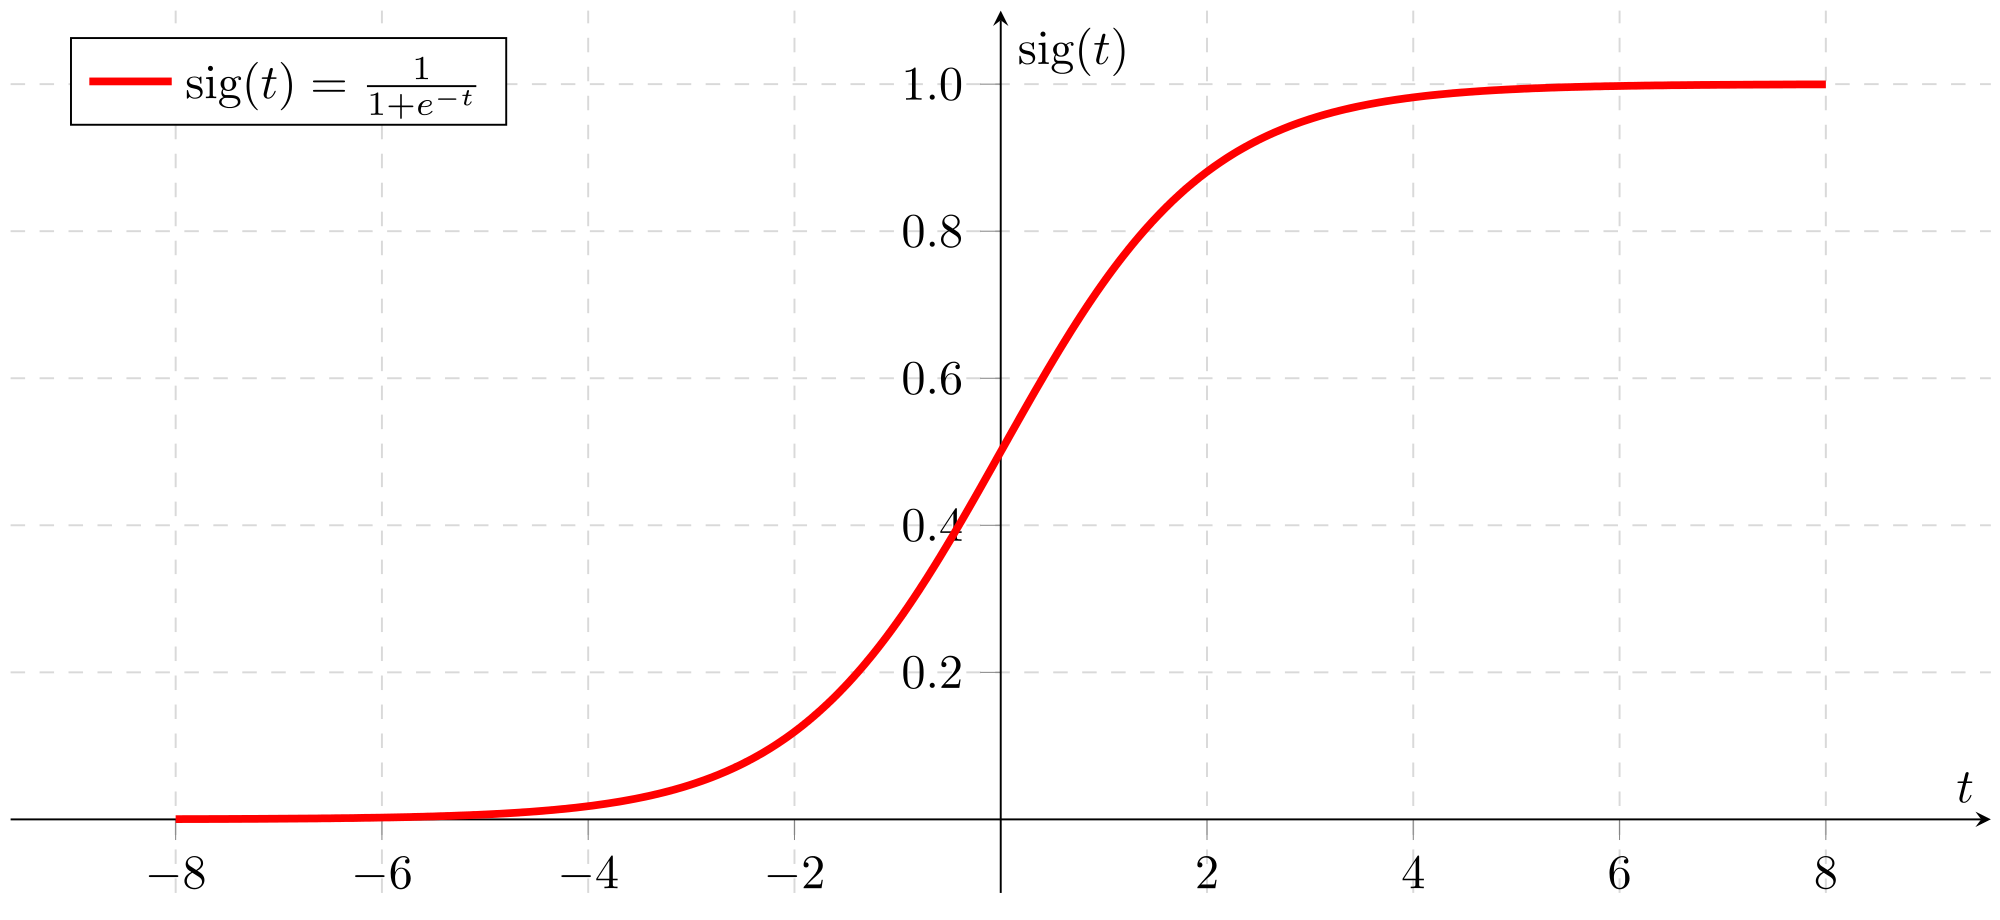
\includegraphics[width=12cm]{Sigmoid.png}
\caption{Sigmoid function}
\label{fig:Sigmoid}
\end{figure}

Interpretation of hypothesis output: $h_\theta(x) = P(y=1|x;\theta)$, ``probability that $y=1$, given $x$, parameterized by $\theta$'', the estimated probability that $y = 1$ on input $x$.

$y \in \{0, 1\}, P(y=0|x;\theta) + P(y=1|x;\theta)=1$

%%
\subsubsection{Decision boundary}

In order to get the discrete 0 or 1 classification, we can translate the output of the hypothesis function as follows:\\
suppose \\ 
predict ``$y=1$'' if $h_\theta(x) \geq 0.5 \Rightarrow \theta^Tx \geq 0$\\
predict ``$y=0$'' if $h_\theta(x) < 0.5 \Rightarrow  \theta^Tx < 0$

\emph{\textcolor{Bittersweet}{The decision boundary is the line that separates the area where $y = 0$ and where $y = 1$. In this case, it's the line or curve of $\theta^TX = 0$  for the binary classification.
% insert figure of the logistic function
Given $\theta$ fitted via a certain procedure, the decision boundary can be plotted in the training data space. The decision boundary is a property, not of the training set, but of the hypothesis under the parameter. The parameters $\theta$ defines the decision boundary. The training set is what we use to fit the $\theta$.}}

\textbf{Non-linear decision boundaries}: $\theta^Tx$ does not have to be linear, similar to the polynomial regression, we could add extra higher order polynomial terms to the features to get complex decision boundaries (e.g., $x_1^2+x_2^2=1$ or a more complex shape).

In a 2-D display, the decision boundary can be plotted as a line (linear, only two features, decided arbitrarily by two $x_1$ points and two $x_2$ points calculated from $X\theta = 0$) or a curve (polynomial, more features created from the $x_{1,2}$ points, contour plot of $X\theta = 0$ on the mesh grid of X).


%%
\subsubsection{Cost function}
\begin{itemize}

\item
Training set: $\{(x^{(1)}, y^{(1)}), (x^{(2)}, y^{(2)}), \cdots, (x^{(m)}, y^{(m)})\}$, m examples\\
$x \in \begin{pmatrix} x_0 \\ x_1 \\ x_2 \vdots \\ x_n \end{pmatrix} \in \mathbb{R}^{n+1}, \quad x_0 = 1, \quad y \in \{0,1\}$

\item
    Cost function \footnote{$h_\theta(x)^y(1-h_\theta(x))^{(1-y)}$}: 
    \begin{align} 
        \text{Cost}(h_\theta(x),y) = \left\{ \begin{array}{rcl}
            -\log(h_\theta(x)) & \mbox{if} & y=1 \\ 
            -\log(1- h_\theta(x)) & \mbox{if} & y=0 \\ \end{array}\right.
    \end{align}
    If  $h_\theta(x)=y$, then cost $(h_\theta(x), y)=0$ for both $y=0$ and $y=1$, see also \textbf{Figure} \ref{fig:costfunction_logisticregressionSVM}\\
    If  $y=0$, then cost $(h_\theta(x), y) \rightarrow \infty$ as $h_\theta(x) \rightarrow 1$\\
    If  $y=1$, then cost $(h_\theta(x), y) \rightarrow \infty$ as $h_\theta(x) \rightarrow 0$\\
    This captures the intuition that if the learning algorithm predicts $P(y=1|x;\theta)=0$, but $y=1$, it will be penalized by a very large cost.
    \begin{align*} 
    J(\theta) = \frac{1}{m}\sum_{i=1}^m\text{Cost}(h_\theta(x^{(i)}), y^{(i)})
    \end{align*}
    Note that $y \in \{0, 1\}$, so we have
    $\text{Cost}(h_\theta(x),y) = -y\log(h_\theta(x)) - (1-y)\log(1- h_\theta(x))$, and
    \begin{align} 
        J(\theta) = -\frac{1}{m}\sum_{i=1}^m \left[ y^{(i)}\log(h_\theta(x^{(i)})) + (1-y^{(i)})\log(1- h_\theta(x^{(i)})) \right]
    \end{align}
    
    A vectorised implementation is:
    \begin{align} 
       h &= g(X\theta)\newline \\
       J(\theta) &= \frac{1}{m} \cdot \left(-y^{T}\log(h)-(1-y)^{T}\log(1-h)\right)
    \end{align}
    
    \emph{\textcolor{Bittersweet}{A particular choice of cost function will give a convex optimisation problem (local optima free). If we take the logistic hypothesis function and plug it in the squared error cost function, it leads to a non-convex function. The gradient descent will not be guaranteed to converge to the global minimum. $J(\theta)$ is in the form of an \textbf{maximum likelihood estimation}.}}
    
\item
    Goal: 
    \begin{itemize}
    \item to fit parameters $\theta$: $\underset{\theta}{\min} \ J(\theta)$\\
    \item to make a prediction given new $x$: Output $P(y=1|x;\theta) = h_{\theta}(x)=\frac{1}{1+e^{-\theta^Tx}}$
    \end{itemize}
    
\item
    Gradient descent:\\
	repeat until convergence \{ \\
	\begin{equation}
	\begin{split}
	\theta_j  = \theta_j - \alpha \frac{1}{m} \sum_{i=1}^m (h_\theta(x^{(i)}) - y^{(i)}) x_j^{(i)}
	\end{split}
	\end{equation}
	(simultaneously update all $\theta_j$)\\
	\}
	
    A vectorized implementation is:
    \begin{align}
    \theta := \theta - \frac{\alpha}{m}X^T(g(X\theta)-y)
    \end{align}
    
    \emph{\textcolor{Bittersweet}{Both linear regression and logistic regression (classification) arrive at the same update rule (identical algorithm), thanks to the design of the cost function (a little calculus exercise, gradient of cross entropy function with sigmoidal probabilities, applying the chain rule and the derivative of logistic function\footnote{$\sigma(z)=\frac{1}{1+e^{-z}}, \diff{\sigma(z)}{z}=\sigma(z)(1-\sigma(z)), \nabla{J(\theta)} = \frac{1}{m}X^T(g(X\theta) - y)$}).}}

\end{itemize}

%
\subsection{Optimization algorithm}
Objective: $\underset{\theta}{\min} J(\theta)$.

For a given input value $\theta$, write a function (code) that compute 
\begin{equation*}
J(\theta), \quad \text{and} \quad \diffp{ }{{\theta_j}} J(\theta)  \quad (\text{for} j=0,1, \cdots, n)
\end{equation*}
and then use an optimization solver.

\begin{itemize}
\item Gradient descent
\item Conjugate gradient
\item BFGS
\item L-BfGS
\end{itemize}

%
\subsection{Multiclass classification: One-vs-all}
One-vs-all (one-vs-rest): take the raining set and turn it into several separate binary classification problems.
Train a logistic regression classifier $h_\theta^{(i)}(x)$ for each class $i$ to predict the probability that $y=i$, for $y \in \{0, 1, \cdots, n\}$. On a new input $x$, to make a prediction, pick the class $i$ that maximizes $h_\theta^{(i)}$, i.g.,  $\text{prediction} = \underset{i}{\max}(h_\theta^{(i)}(x))$. Example: 3 classes. We take one class and then lump all the others into a single second class, repeatedly applying binary logistic regression to each class, e.g., class one gets assigned to the positive class, and classes two and three get assigned to the negative class (fake training set).

%
\subsection{Regularization}
Regularization allows us to ameliorate (reduce) the overfitting problem.\\
\begin{itemize}
\item
``Underfitting'': high bias (preconception, hypothesis too simple, too few features)
\item
``Overfitting'': high variance (unnecessarily complicated hypothesis, fail to \textbf{generalize} to new examples)
\item
``Just right''
\end{itemize}

Addressing overfitting:

\begin{itemize}
\item
reduce number of features.
	\begin{itemize}
	\item manualluy select which features to keep
	\item Model selection algorithm
	\end{itemize}
	
\item
Regularization
\begin{itemize}
	\item Keep all the features, but reduce magnitude/values of parameter $\theta_j$, when there are a lot of slightly useful features.
	\end{itemize}
\end{itemize}

%%
\subsubsection{Cost function}
\underline{Intuition}:\\
Small values for parameters $\theta_0, \theta_1, \cdots, \theta_n$ leads to ``simpler'' hypothesis, smoother function, less prone to overfitting.\\
\underline{Example}:\\
Features: $x_0, x_1, \cdots, x_n$\\
Parameters: $\theta_0, \theta_1, \cdots, \theta_n$ 

To modify the linear regression cost function to shrink all the parameters by \textbf{adding an extra regularization term}
\begin{align}
\underset{\theta}{\min}\frac{1}{2m} \left[ \sum_{i=1}^m(h_\theta(x^{(i)})-y^{(i)})^2 + \lambda \sum_{j=1}^n\theta_j^2 \right]
\end{align}
$\lambda$: regularization parameter. It controls a tradeoff between the goal of fitting the training set well and the goal of keeping the parameters small (keeping the hypothesis simple). In regularized linear regression, if $\lambda$ is set too large, e.g., $\lambda = 10^{10}$, then $\theta_{1, 2, \cdots, n} \approx 0, h_{\theta_0}=\theta_0$, which may smooth out the function too much and cause ``underfit''. If $\lambda$ is set too small, the classifier gets almost every training example correct, but draws a very complicated boundary, thus ``overfitting'' the data.

%%
\subsubsection{Regularized linear regression}

\underline{Gradient descent}\\
repeat until convergence \{ \\
\begin{align*} 
\theta_0: &= \theta_0 - \alpha \frac{1}{m} \sum_{i=1}^m (h_\theta(x^{(i)}) - y^{(i)})x_0^{(i)}\\
\theta_j: &= \theta_j - \alpha \left[ \frac{1}{m} \sum_{i=1}^m ((h_\theta(x^{(i)}) - y^{(i)})x^{(i)}_j) + \frac{\lambda}{m}\theta_j \right]\\
	     &= \theta_j(1-\alpha\frac{\lambda}{m}) - \frac{\alpha}{m} \sum_{i=1}^m ((h_\theta(x^{(i)}) - y^{(i)})x^{(i)}_j)
&(j=1, 2, 3, \cdots, n)
\end{align*}
\}\\
Regularization is not added to $\theta_0$.\\
$\theta_{1, \cdots, n}$ is penalized (reducing its value by some amount on every update). usually $1-\alpha\frac{\lambda}{m} < 1$, slightly smaller than 1.\\
\underline{Normal equation}\\
\begin{align*}
X = \begin{pmatrix} (x^{(i)})^T \\ \vdots \\ (x^{(m)})^T \end{pmatrix}, \quad y = \begin{pmatrix} y^{(i)} \\ \vdots \\ y^{(m)} \end{pmatrix}
\end{align*}
to $\underset{\theta}{\min}J(\theta)$,\\
\begin{align}
\theta = (X^TX + \lambda
\begin{bmatrix}
   0 &  &  & \\ 
   & 1 &  & \\ 
   &  &  \ddots & \\ 
   &  &   & 1
\end{bmatrix})^{-1}X^Ty
\end{align}
If $m<n$, then $X^TX$ is non-invertible.
However when $\lambda > 0$, $X^TX+\lambda \cdot L$ becomes invertible, where 
$L = \begin{bmatrix}
   0 &  &  & \\ 
   & 1 &  & \\ 
   &  &  \ddots & \\ 
   &  &   & 1
\end{bmatrix} \in \mathbb{R}^{(n+1)\times(n+1)}$

%%
\subsubsection{Regularized logistic regression}

\underline{Cost function}
   \begin{align} 
        J(\theta) &= -\frac{1}{m}\sum_{i=1}^m \left[ y^{(i)}\log(h_\theta(x^{(i)})) + (1-y^{(i)})\log(1- h_\theta(x^{(i)})) \right] + \frac{\lambda}{2m}\sum_{j=1}^n\theta_j^2 \\
        &(j=1, 2, 3, \cdots, n) \nonumber
    \end{align}
Note that $\theta_0$ is explicitly excluded in the regularization term.

\underline{Gradient descent}\\
repeat until convergence \{ \\
\begin{align*} 
\theta_0: &= \theta_0 - \alpha \frac{1}{m} \sum_{i=1}^m (h_\theta(x^{(i)}) - y^{(i)})x_0^{(i)}\\
\theta_j: &= \theta_j - \alpha \left[\frac{1}{m} \sum_{i=1}^m ((h_\theta(x^{(i)}) - y^{(i)})x^{(i)}_j) + \frac{\lambda}{m}\theta_j \right]\\
&(j \in {1, 2, 3, \cdots, n})
\end{align*}
\}\\

\underline{A vectorised implementation} is:\\
\begin{align*}
X = \begin{pmatrix} 
    1 & x_1^1 & x_2^1 & \cdots & x_n^1 \\
    1 & x_1^2 & x_2^2 & \cdots & x_n^2 \\
    \vdots &&&& \vdots \\
    1 & x_1^m & x_2^m & \cdots & x_n^m \\
     \end{pmatrix} 
\in \mathbb{R}^{m \times (n+1)},
L = \begin{bmatrix}
   0 &  &  & \\ 
   & 1 &  & \\ 
   &  &  \ddots & \\ 
   &  &   & 1
\end{bmatrix}
\in \mathbb{R}^{(n+1)\times(n+1)},
\theta = \begin{pmatrix} \theta_0 \\ \theta_1 \\ \theta_2 \vdots \\ \theta_n \end{pmatrix}
\in \mathbb{R}^{n+1}
\end{align*}

\begin{align} 
h &= g(X\theta) \nonumber \\
J(\theta) &= \frac{1}{m} \cdot \left(-y^{T}\log(h)-(1-y)^{T}\log(1-h)\right) +\frac{\lambda}{2m}(L\cdot\theta)^T(L\cdot\theta)\\
\diffp{J(\theta)}{\theta} &= \frac{1}{m}X^T(h_\theta(x)-y) + \frac{\lambda}{m}(L\cdot\theta)
\end{align}

%_________________________________________________________________
\section{Neural Networks}
\label{sec:Neural Networks}
%
\subsection{Non-linear hypothesis and neurons in the brain}
The problem of learning complex non-linear hypotheses: The number of features (e.g., all polynomial terms) very rapidly becoms unwieldy and impractical. Neural networks offers an alternate way to perform machine learning when we have complex hypotheses with many features.

Example: a grid of pixel intensity values. $50 \times 50$ pixel images $\rightarrow 2500$ pixels in grey scale (750 if RGB), $n=2500$. In this case, a nonlinear hypothesis by including all the the quadratic features $x_i \times x_j$ would end up a total of 3 million features \footnote{The number of new features for all polynomial terms: $\frac{(n+r-1)!}{r!(n-1)!}$. $n =$ the number of original features; $r =$  the polynomial order. e.g., quadratic: $\mathcal{O}(n^2/2)$; cubic: $\mathcal{O}(n^3)$}.

Neural networks were developed as simulating neurons or networks of neurons in the brain. The ``one learning algorithm'' hypothesis: Neuro-rewiring experiments at the 20s.
%
\subsection{Model representation}
%%
\subsubsection{Neuron model: Logistic unit}
\underline{Input}: $x$ (features $x_1, x_2, \cdots, x_n$).\\ 
\underline{Output}: $h_\theta(x)=\frac{1}{1+e^{-\theta^{T}x}}$ (result of the hypothesis function).\\
\underline{Terminology}: $x_0=1$: bias unit; Sigmoid (logistic) activation function $g(z) = \frac{1}{1+e^{-z}}$; Parameters of the model $\theta$: Weights; The first layer: Input layer; Intermediate layers: Hidden layer; The last layer: Output layer; Architecture: How the different neurons are connected to each other.\\

The intermediate``hidden'' layer:\\
$a_j^{(l)} = $``activation'' of unit $j$ in layer $l$\\
$\Theta^{(l)} = $ matrix of weights controlling function mapping from layer $l$ to layer $l+1$\\

The values for each of the ``activation'' nodes in a model with only one hidden layer:
\begin{align*}
a_1^{(2)}&=g(\Theta_{10}^{(1)}x_0+\Theta_{11}^{(1)}x_1+\Theta_{12}^{(1)}x_2+\Theta_{13}^{(1)}x_3)\\
a_2^{(2)}&=g(\Theta_{20}^{(1)}x_0+\Theta_{21}^{(1)}x_1+\Theta_{22}^{(1)}x_2+\Theta_{23}^{(1)}x_3)\\
a_3^{(2)}&=g(\Theta_{30}^{(1)}x_0+\Theta_{31}^{(1)}x_1+\Theta_{32}^{(1)}x_2+\Theta_{33}^{(1)}x_3)\\
h_{\Theta}(x)&=a_1^{(3)}=g(\Theta_{10}^{(2)}a_0^{(2)}+\Theta_{11}^{(2)}a_1^{(2)}+\Theta_{12}^{(2)}a_2^{(2)}+\Theta_{13}^{(2)}a_3^{(2)})
\end{align*}
Each layer gets its own matrix of weights, $\Theta^{(l)}$\\
If network has $s_l$ units in layer $l$ and $s_{l+1}$ units in layer $l+1$, then $\Theta^{(l)}$ will be of dimension $s_{l+1} \times (s_{l}+1)$. The $+1$ comes from the addition in $\Theta^{(l)}$ of the ``bias nodes'' $\Theta^{(l)}_0$ for $x_0$.

%%
\subsubsection{Forward propagation: Vectorized implementation}

\underline{Example}:\\
$a^{(1)} = x = \begin{pmatrix} x_0 \\ x_1 \\ x_2 \\ x_3 \end{pmatrix} \in \mathbb{R}^{4}$, \quad
$z = \begin{pmatrix} z_1 \\ z_2 \\ z_3 \end{pmatrix} \in \mathbb{R}^{3}$\\
\begin{align*}
z^{(2)} &= \Theta^{(1)}a^{(1)}\\
a^{(2)} &= g(z^{(2)}), \quad \text{add} \quad a^{(2)}_0 = 1\\
z^{(3)} &= \Theta^{(2)}a^{(2)}\\
h_{\Theta}(x) &= a^{(3)} = g(z^{(3)})
\end{align*}

The vector representation:\\
$a^{(1)} = x = \begin{pmatrix} x_0 \\ x_1 \\ \vdots \\ x_n \end{pmatrix} \in \mathbb{R}^{(n+1)}$, \quad
$z^{(l)} = \begin{pmatrix} z^{(l)} _1 \\ z^{(l)} _2 \\ \vdots \\ z^{(l)} _n \end{pmatrix} \in \mathbb{R}^{n}$\\
\begin{align*}
z^{(l)} &= \Theta^{(l-1)}a^{(l-1)}\\
a^{(l)} &= g(z^{(l)}), 
\end{align*}

Rather than using the original features $x$, the model is using new features $a^{(2, \cdots, l+1)}$, which are learned as functions of the values of the activation nodes. Neural network learns its own features $a^{(2, \cdots, l+1)}$ of the hidden layers.

%%
\subsubsection{Examples: Simulating logical gates}
\underline{Example}: AND \footnote{$ g(x)=\frac{1}{1+e^{-z}}, z = 4.6, g = 0.99; z = -4.6, g = 0.01 $}\\
\begin{align*}
x_1, x_2 & \in \{0,1\}, x_0 = 1\\
y &= x_1~\text{AND}~x_2\\
h_\Theta(x) &= g(\Theta_{10}^{(1)}x_0 + \Theta_{11}^{(1)} x_1 + \Theta_{12}^{(1)}x_2)\\
&= g(-30 + 20x_1 +20x_2) 
\end{align*}
\\\\
\underline{Example}: OR \quad $h_\Theta(x) = g(-10 + 20x_1 +20x_2)$\\
\\\\
\underline{Example}: Negation \quad $h_\Theta(x) = g(10 - 20x_1)$\\
\\\\
\underline{Example}: (NOT $x1$) AND (NOT $x_2$)) \quad $h_\Theta(x) = g(30 - 20x_1- 20x_2)$\\
\\\\
\underline{Example}: XNOR
\begin{align*}
\begin{bmatrix} x_0\\x_1\\x_2 \end{bmatrix}
\rightarrow
\begin{bmatrix} a_1^{(2)}\\a_2^{(2)} \end{bmatrix} 
\rightarrow
\begin{bmatrix} a^{(3)}\end{bmatrix} 
\rightarrow
h_\Theta(x)
\end{align*}
\begin{align*}
a^{(2)} &= g(\begin{bmatrix}-30 & 20 & 20\\ 10 & -20 & -20\end{bmatrix} \cdot \begin{bmatrix} x_0\\ x_1\\ x_2 \end{bmatrix})\\
h_\Theta(x) &= g(\begin{bmatrix}-10 & 20 & 20\end{bmatrix}) \cdot a^{(2)}
\end{align*}

%%
\subsubsection{Multiclass classification}
Multiple output units: One-vs-all.\\
\underline{Example}: 4 categories.\\
$h_\Theta(x) \approx y^{i} \in \begin{pmatrix}
\begin{bmatrix} 1\\ 0\\ 0\\ 0\end{bmatrix}, \begin{bmatrix} 0\\ 1\\ 0\\ 0\end{bmatrix}, \begin{bmatrix} 0\\ 0\\ 1\\ 0\end{bmatrix}, \begin{bmatrix} 0\\ 0\\ 0\\ 1\end{bmatrix}
\end{pmatrix}$

%
\subsection{Cost function}
Neural network classification:

\begin{center}
\begin{tabular}{| l | l | l |}
\hline
Binary classification & Multi-class classification (K classes)\\
\hline
$y \in {0,1}$  &
$y \in \mathbb{R}^K$ e.g., $\begin{pmatrix}
\begin{bmatrix} 1\\ 0\\ 0\\ 0\end{bmatrix}, \begin{bmatrix} 0\\ 1\\ 0\\ 0\end{bmatrix}, \begin{bmatrix} 0\\ 0\\ 1\\ 0\end{bmatrix}, \begin{bmatrix} 0\\ 0\\ 0\\ 1\end{bmatrix}
\end{pmatrix}$ \\
1 output unit & K output units\\
\hline
\end{tabular}
\end{center}

\begin{itemize}
\item
variables:
    \begin{itemize}
        \item
        $\{(x^{(1)}, y^{(1)}), (x^{(2)}, y^{(2)}), \cdots, (x^{(m)}, y^{(m)})\}$
        \item
        $L = $ total number of layers in network
        \item
        $s_l = $ number of units (not counting the bias unit) in layer $l$
        \item
        $K = $ number of output units/classes
    \end{itemize}
\item
Cost function\\
Logistic regression:\\
   \begin{align*} 
        J(\theta) = -\frac{1}{m}\sum_{i=1}^m \left[ y^{(i)}\log(h_\theta(x^{(i)})) + (1-y^{(i)})\log(1- h_\theta(x^{(i)})) \right] + \frac{\lambda}{2m}\sum_{j=1}^n\theta_j^2
    \end{align*}
Neural network:\\
   \begin{align} 
   & h_\Theta(x) \in \mathbb{R}^K, \quad  (h_\Theta(x))_k = k^{th} \text{output } \nonumber \\
        J(\Theta) &= -\frac{1}{m} \sum_{i=1}^m\sum_{k=1}^{K} \left[ y_k^{(i)}\log(h_\Theta(x^{(i)}))_k + (1-y^{(i)}_k)\log(1- h_\Theta(x^{(i)}))_k \right] + \notag \\ &\qquad
         \frac{\lambda}{2m}\sum_{l=1}^{L-1}\sum_{i=1}^{s_l}\sum_{j=1}^{s_{l+1}}(\Theta_{j,i}^{(l)})^2
    \end{align}
\end{itemize}

\emph{\textcolor{Bittersweet}{The regulation term adds up the squares of all the individual $\Theta$s in the entire network.}}

%
\subsection{Backpropagation algorithm}
``Backpropagation'' is neural-network terminology for minimizing the cost function.\\
Gradient computation:\\
$\delta_j^{(l)} = $ ``error'' of node $j$ in layer $l$.\\
\newline
Set $\Delta_{ij}^{(l)} = 0$ for all $l, i, j$.\\
For training example $i = 1$ to $m$

\begin{enumerate}
\item
Set $a^{(1)} := x^{(1)}$
\item
Perform forward propagation to compute $a^{(l)}$ for $l=2,3, \cdots, L$\\
using $z^{(j)} = \Theta^{(j-1)}a^{(j-1)}, a^{(j)} = g(z^{(j)})$
\item
Using $y^{(i)}$, compute $\delta^{(L)} = a^{(L)}-y^{(i)}$ (the ``error values'' for the last layer)\\
$L = $ total number of layers\\
$a^{(L)} = $ the vector of outputs of the activation 
\item
Compute $\delta^{(L-1)}, \delta^{(L-2)}, \cdots, \delta^{(2)}$\\
using $\delta^{(l)} = ((\Theta^{(l)})^T \delta^{(l+1)})) \odot a^{(l)} \odot (1-a^{(l)})$ \footnote{$\odot$: elment-wise multiplication; $g'(z^{(l)}) = a^{(l)} \odot (1-a^{(l)})$}
\item
$\Delta_{ij}^{(l)} := \Delta_{ij}^{(l)} + a_j^{(l)}\delta_i^{(l+1)}$\\
(Vectorized implementation:
$\Delta^{(l)} := \Delta^{(l)} + \delta^{(l+1)}(a^{(l)})^T$)
\end{enumerate}

\begin{align}
D_{ij}^{(l)} &:= \frac{1}{m} \left(\Delta_{ij}^{(l)} + \lambda\Theta_{ij}^{(l)}\right) \qquad \text{if} j \neq 0 \nonumber\\
D_{ij}^{(l)} &:= \frac{1}{m}\Delta_{ij}^{(l)} \qquad \text{if} j = 0\\
&\frac{\partial}{\partial{\Theta_{ij}^{(l)}}} J(\Theta) =  D_{ij}^{(l)}
\end{align}

%%
\subsubsection{Implementation notes}
\begin{itemize}
\item
    Unrolling parameters:\\
    \underline{Example}:\\
    \begin{align*}
    &s_1 = 10, s_2 = 10, s_3 = 1\\
    &\Theta^{(1)} \in \mathbb{R}^{10 \times 11}, \Theta^{(2)} \in \mathbb{R}^{10 \times 11}, \Theta^{(3)} \in \mathbb{R}^{1 \times 11}\\
    &D^{(1)} \in \mathbb{R}^{10 \times 11}, D^{(2)} \in \mathbb{R}^{10 \times 11}, D^{(3)} \in \mathbb{R}^{1 \times 11}
    \end{align*}
    ``unroll'' all the elements in the matrices and put them into one long vector.
\item
    Numerical gradient checking:\\
    \begin{align*}
    \diff{J(\theta)}{\theta} & \approx \frac{J(\theta + \varepsilon)-J(\theta - \varepsilon)}{2 \varepsilon}\\
    \diff{J(\theta)}{{\theta_j}} & \approx \frac{J(\theta_1, \cdots, \theta_j + \varepsilon, \cdots, \theta_n)-J(\theta_1, \cdots, \theta_j - \varepsilon, \cdots, \theta_n)}{2 \varepsilon}
    \end{align*}
    $\theta \in \mathbb{R}^n$, e.g., the ``unrolled'' version of $\Theta$. e.g., $\varepsilon = 10^{-4}$
\item
    Initial value of $\Theta$:
    
    $\Theta_{ij}^{(l)} = 0$ for al $i, j, l$. After each update, parameters corresponding to inputs going into each of the hidden units are identical.

    Random initialization (Symmetry breaking):\\
    Initialize each $\Theta_{ij}^{(l)}$ to a random value in $[-\epsilon, \epsilon]$, i.e., $-\epsilon \leq \Theta_{ij}^{(l)} \leq \epsilon$\\
    e.g., $\epsilon = \frac{\sqrt{6}}{\sqrt{s_l + s_{l+1}}}$ for $\Theta^{(l)}, \Theta^{(l)} = 2\epsilon~\text{rand}(s_{(l+1)}, (s_{l}+1))-\epsilon$
\end{itemize}

%
\subsection{Training a neural network}

\begin{itemize}
\item
Pick a network architecture
    \begin{itemize}
    \item
    Number of input units: Dimension of features $x^{(i)}$
    \item
    Number of output units: Number of classes\\
    $y \in \{1, 2, \cdots, n\} \rightarrow y \in \begin{pmatrix}
    \begin{bmatrix} 1\\ 0\\ 0\\ 0 \\ \vdots \\ 0\end{bmatrix}, \begin{bmatrix} 0\\ 1\\ 0\\ 0 \\  \vdots \\ 0\end{bmatrix}, \begin{bmatrix} 0\\ 0\\ 1\\ 0 \\  \vdots \\ 0 \end{bmatrix}, \cdots, \begin{bmatrix} 0\\ 0\\ 0\\ 0 \\  \vdots \\ 1 \end{bmatrix}
    \end{pmatrix}$
    \item
    Number of hidden units per layer = usually more the better, but must balance with the cost of computation.
    \end{itemize}
Reasonable default: For 1 hidden layer, or if more than 1 hidden layer, have same number of hidden units in every layer.

\item
    Training
    \begin{enumerate}
        \item
        Randomly initialize the weights
        \item
        Implement forward propagation to get $h_{\Theta}(x^{(i)})$ for any $x^{(i)}$
        \item
        Implement code to compute cost function $J(\Theta)$
        \item
        Implement backprop to to compute partial derivatives $\frac{\partial}{\partial{\Theta_{ij}^{(l)}}} J(\Theta)$
        \item
        Use gradient checking to compare $\frac{\partial}{\partial{\Theta_{ij}^{(l)}}} J(\Theta)$ computed using backpropagation vs. using numerical estimate of gradient of $J(\Theta)$. Then disable gradient checking.
        \item
        Use gradient descent or advanced optimization method with backpropagation to try to minimize $J(\Theta)$ as a function of parameters $\Theta$
        
        \emph{\textcolor{Bittersweet}{$J(\Theta)$ is non-conves, it is susceptible to local minima}}
    \end{enumerate}    
\item
A vectorised implementation\\
\begin{align*}
&X = \begin{pmatrix} 
    1 & x_1^1 & x_2^1 & \cdots & x_n^1 \\
    1 & x_1^2 & x_2^2 & \cdots & x_n^2 \\
    \vdots &&&& \vdots \\
    1 & x_1^m & x_2^m & \cdots & x_n^m \\
     \end{pmatrix} 
\in \mathbb{R}^{m \times (n+1)}\\
&Y = \begin{bmatrix}
   \begin{bmatrix} 1\\ 0\\ 0\\ 0 \\ \vdots \\ 0\end{bmatrix}, \begin{bmatrix} 0\\ 1\\ 0\\ 0 \\  \vdots \\ 0\end{bmatrix}, \begin{bmatrix} 0\\ 0\\ 1\\ 0 \\  \vdots \\ 0 \end{bmatrix}, \cdots, \begin{bmatrix} 0\\ 0\\ 0\\ 0 \\  \vdots \\ 1 \end{bmatrix}
\end{bmatrix}
\in \textbf{Boolean}^{(m)\times(K)}\\
&\Theta^{(j)} \in \mathbb{R}^{s_{(l+1)} \times (s_l +1)}\\
&a^{(l)} = g(a^{(l-1)}{(\Theta^{(l-1)})}^{T})\\
&a^{(l)} = [\text{ones}(m,1), a^{(l)}]\\
&h_{\Theta}(X) = a^{(L)}\\
&\theta = \text{``unroll''} \quad \Theta^{(1, \cdots, L)}(:, 2:(s_l+1))
\end{align*}
\begin{align} 
&J(\theta) = \frac{1}{m} \cdot \sum(\left(-Y \odot \log(h) - (1-Y) \odot \log(1-h)\right)) +\frac{\lambda}{2m}\theta^T\theta\\
&\delta^{(L)} = a^{(L)}-Y\\
&\delta^{(l)} = (\delta^{(l+1)}\Theta^{(l)})) \odot a^{(l)} \odot (1-a^{(l)})\\
&\delta^{(l)} = \delta^{(l)}(:, 2:end)\\
&\Theta^{(l)}(:,1) = 0\\
&D^{(l)} = \frac{1}{m}(\delta^{(l+1)})^{T}a^{(l)} + \frac{\lambda}{m}\Theta^{(l)}
\end{align}
\end{itemize}

%_________________________________________________________________
\section{Machine learning diagnostic}
\label{sec:Machine learning diagnostic}
%
\subsection{debugging a learning algorithm (trouble shooting)}
\begin{itemize}
\item
get more training examples $\rightarrow$ fixes high variance
\item
try smaller sets of features $\rightarrow$ fixes high variance
\item
try getting additional features $\rightarrow$ fixes high bias
\item
try adding polynomial features $\rightarrow$ fixes high bias
\item
try increasing or decreasing $\lambda$ $\rightarrow$ fixes high bias/variance
\end{itemize}

%
\subsection{Evaluating a hypothesis}
Training/testing procedure:\\
Learning parameter $\Theta$ from training data (minimizing training error $J_{\text{train}}(\Theta)$)\\
Compute test set error $J_{\text{test}}(\Theta)$) (e.g., split up the data: Training set (random 70\%) vs. Test set (random 30\%)):
\begin{itemize}
\item
for linear regression

$J_{\text{test}}(\Theta) = \frac{1}{2m_{\text{test}}} \sum_{i=1}^{m_{\text{test}}}(h_\Theta(x_{\text{test}}^{(i)}) - y_{\text{test}}^{(i)})^{2}$
\item
for logistic regression

$J_{\text{test}}(\Theta) = -\frac{1}{2m_{\text{test}}}\sum_{i=1}^{m_{\text{test}}}(y_{\text{test}}^{(i)} \log h_\Theta(x_{\text{test}}^{(i)}) + (1-y_{\text{test}}^{(i)})\log(1-h_\Theta(x_{\text{test}}^{(i)}))$
\item
Misclassification error (0/1 misclassification error):
\begin{align}
err(h_\Theta(x), y) &= \left\{ \begin{array}{rll}
         1 & \text{if} \quad h_\Theta(x) \geq 0.5, y = 0;\\
            & \text{or if} \quad h_\Theta(x) \leq 0.5, y = 1.\\
         0 & \text{otherwise}
                \end{array}\right.\\
\text{Test error} &= \frac{1}{m_\text{{test}}}\sum_{i = 1}^{m_\text{{test}}}err(h_\Theta(x_{\text{test}}^{(i)}, y_{\text{test}}^{(i)})
\end{align}
The proportion of the test data that was misclassified.
\end{itemize}

% 
\subsection{Model selection and train/validation/test sets}
Just because a learning algorithm fits a training set well, that doesn't mean it's a good hypothesis. The training error is likely to be lower than the actual generalization error.
\\\\
\underline{Example} Given many models with different polynomial degrees:
split the data into: e.g., Training set (random 60\%); Cross validation set (random 20\%); Test set (random 20\%).
\begin{itemize}
\item
Training error: $J(\Theta)$, optimize the parameters $\Theta$ using the training set for each polynomial degree.
\item
Cross validation error: $J_{\text{cv}}(\Theta)$, find the polynomial degree $d$ with the least error using the cross validation set. Pick the hypothesis with the lowest cross validation error. 
\item
Test error: $J_{\text{test}}(\Theta^{(d)})$
The test set is then used to estimate the generalization error of the model that was selected.
\end{itemize}

% 
\subsection{Diagnosing bias vs. variance}
Training error: $J_{\text{train}}(\Theta) = \frac{1}{2m_{\text{train}}} \sum_{i=1}^{m_{\text{train}}}(h_\Theta(x_{\text{train}}^{(i)}) - y_{\text{train}}^{(i)})^{2}$\\
Cross validation error: $J_{\text{cv}}(\Theta) = \frac{1}{2m_{\text{cv}}} \sum_{i=1}^{m_{\text{cv}}}(h_\Theta(x_{\text{cv}}^{(i)}) - y_{\text{cv}}^{(i)})^{2}$\\

High bias: underfitting; $J_{\text{train}}{\Theta} \approx J_{\text{cv}}{\Theta}$

High variance: overfitting; $J_{cv}{\Theta} \gg J_{\text{train}}{\Theta}$\\

\begin{figure}[h]
\centering
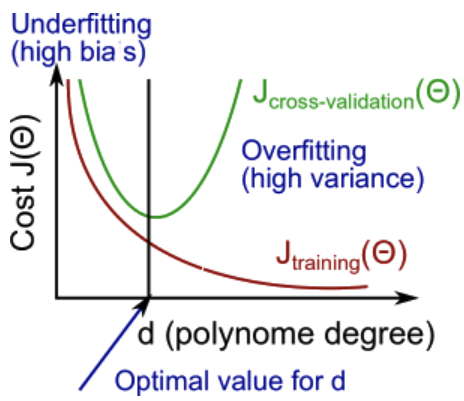
\includegraphics[width=6.5cm]{Bias_Variance}
\caption{Training error vs. Cross validation error}
\label{fig:BiasvsVariance}
\end{figure}
\underline{Bias-variance tradeoff}: Models with high bias are not complex enough for the data and tend to underfit, while models with high variance might overfit the training data.

%%
\subsubsection{Regularization and Bias/Variance}
Linear regression with regularization
\begin{flalign*}
\text{Model}: h_\Theta(x) &= \Theta_0 + \Theta_1x + \Theta_2x^2 +\Theta_3x^3 +\Theta_4x^4\\
J(\Theta) &= \frac{1}{m}\sum_{i=1}^m(h_\Theta(x^{(i)}) - y^{(i)})^2 + \frac{\lambda}{2m}\sum_{j=1}^{n}\Theta_j^2\\
J_{\text{train}}(\Theta) &= \frac{1}{2m_{\text{train}}} \sum_{i=1}^{m_{\text{train}}}(h_\Theta(x_{\text{train}}^{(i)}) - y_{\text{train}}^{(i)})^{2}\\
J_{\text{cv}}(\Theta) &= \frac{1}{2m_{\text{cv}}} \sum_{i=1}^{m_{\text{cv}}}(h_\Theta(x_{\text{cv}}^{(i)}) - y_{\text{cv}}^{(i)})^{2}\\
J_{\text{test}}(\Theta) &= \frac{1}{2m_{\text{test}}} \sum_{i=1}^{m_{\text{test}}}(h_\Theta(x_{\text{test}}^{(i)}) - y_{\text{test}}^{(i)})^{2}
\end{flalign*}

\begin{figure}[h]
\centering
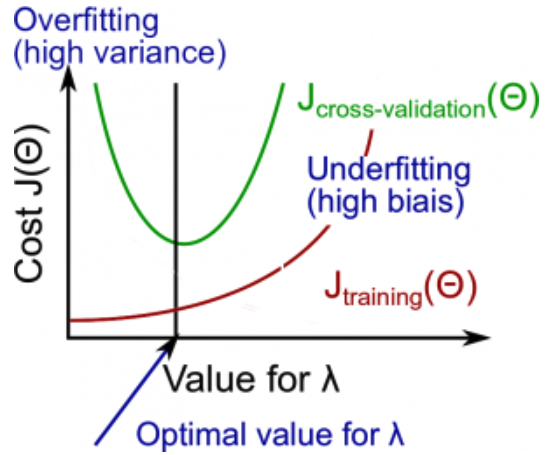
\includegraphics[width=6.5cm]{Bias_Variance_Regularization}
\caption{Regularization and the hypothesis}
\label{fig:BiasvsVariance_Regularization}
\end{figure}

How to automatically choose a good regularization parameter $\lambda$?

Try $\lambda = \{0, 0.01, 0.02, 0.04, \cdots, 10 \} \rightarrow \min{J(\Theta)} \rightarrow \Theta \rightarrow J_{\text{cv}}(\Theta) \rightarrow J_{\text{test}}(\Theta)$\\
$J_{\text{cv}}(\Theta)$ without regularization ($\lambda = 0$). 

The training set is used to learn the model parameters $\theta$ at a given $\lambda$. The cross validation set is used to evaluate how good each $\lambda$ value is and the best $\lambda$ is selected accordingly. 
\begin{itemize}
\item
large $\lambda$: high bias (underfit)
\item
intermediate $\lambda$: ``just right''
\item
small $\lambda$: high variance (overfit)
\end{itemize}

%%
\subsubsection{Learning curves}
If a learning algorithm is suffering from high bias, getting more training data will not help much.\\
If a learning algorithm is suffering from high variance, getting more training data is likely to help.\\
Plotting learning curves can often help figure out the problem suffering by the algorithm.
\begin{figure}[h]
\centering
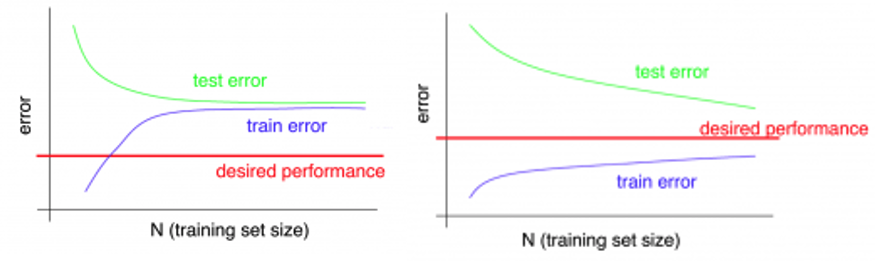
\includegraphics[width=14cm]{Bias_Variance_LearningCurve}
\caption{Typical learning curve for high bias (left) and high variance (right) at fixed model complexity}
\label{fig:BiasvsVarianceLearningCurve}
\end{figure}

%_________________________________________________________________
\section{Machine learning system design}
\label{sec:Machine learning system design}
%
\subsection{Prioritizing what to work on}
\underline{Example}: Building a spam classifier

Supervised learning.\\
$x = $ features of email. $y = $ spam (1) or not spam (0).\\
Features $x$: Choose 100 words indicative of spam/not spam $\rightarrow$ encode it into a feature vector, $x \in \mathbb{R}^{100}$
\begin{align*}
x_j = \left\{ \begin{array}{rll}
         1 & \text{if word} \quad j \quad \text{appears in the email}\\
         0 & \text{otherwise}
                \end{array}\right.\\
\end{align*}
In practice, take most frequently occurring $n$ words (10,000 to 50,000) in training set, rather that manually pick 100 words.
How to spend your time to make it have low error?
\begin{itemize}
\item
Collect lots of data, e.g., ``honeypot'' project, but doesn't always work
\item
Develop sophisticated features based on email routing information (from email header)
\item
Develop sophisticated features for message body, e.g., ``discount'' vs. ``discounts'', ``deal'' vs. ``Dealers''
\item
Develop sophisticated algorithm to detect misspellings
\end{itemize}

%
\subsection{Error analysis}
\begin{itemize}
\item
Start with a simple algorithm, implement it quickly, and test it early on the cross validation data, e.g., quick and dirty running to see if the different ideas are improving the performance of the algorithm, to decide what to fold in and to incorporate into the learning algorithm.
\item
plot learning curves of training and test errors to figure out what problems the learning algorithms suffer, e.g., more data, more features are likely to help. ``premature optimization''.
\item
Error analysis: manually examine the examples (in the cross validation set) that the algorithm made errors on. See if you spot any systematic trend in what type of examples it is making errors on.\\
\underline{Example} spam classifier: what type of email it is; what cues (features) you think would have helped the algorithm classify them correctly.\\
\underline{Numerical evaluation}, e.g., a single real number evaluation metric, cross validation error, accuracy, error.\\
``stemming'' software. e.g., ``Porter stemmer''.
\end{itemize}

%
\subsection{Error metrics for skewed classes}
\underline{Example}: Cancer classification example. Train logistic regression model $h_\theta(x)$. ($y=1$ if cancer, $y=0$ otherwise)\\
got $1\%$ error on test set.\\
only 0.5\% patients have cancer\\
skewed classes: a lot of more examples from one class than the other class. It becomes much harder to use classification accuracy.\\

%%
\subsubsection{Precision/recall} 
as an evaluation metric for classification problems with skewed classes.\\

$y = 1$ in presence of \underline{rare} class to be detected.
\begin{center}
\begin{tabular}{ r|c|c| }
\multicolumn{1}{r}{}
 &  \multicolumn{1}{c}{Actual 1}
 & \multicolumn{1}{c}{Actual 0} \\
\cline{2-3}
Predicted 1& True positive & False positive \\
\cline{2-3}
Predicted 0 & False negative & True negative \\
\cline{2-3}
\end{tabular}
\end{center}

\textbf{Precision}

$\frac{\text{True positives}}{\sharp \text{predicted as positive}} = \frac{\text{True positives}}{\text{True positives + False positives}}$\\

\textbf{Recall}

$\frac{\text{True positives}}{\sharp \text{actual positives}} = \frac{\text{True positives}}{\text{True positives + False negatives}}$\\

If a classifier is getting high precision and high recall, we are confident that the algorithm has to be doing well, even if we have very skewed classes.

%%
\subsubsection{Trading off precision and recall}
Logistic regression: $0 \leq h_\theta(x) \geq 1$\\
Predict 1 if $h_\theta(x) \geq 0.5 \rightarrow 0.7, 0.9, 0.3$\\
Predict 0 if $h_\theta(x) < 0.5 \rightarrow 0.7, 0.9, 0.3$\\

To control the trade-off by choosing the threshold parameter.\\
Suppose we want to predict $y = 1$ (cancer) only if very confident.

$\rightarrow$ Higher precision, lower recall\\
Suppose we want to avoid missing too many cases of cancer (avoid false negatives).

$\rightarrow$ Higher recall, lower precision\\

\textbf{$F_1$ Score} for comparing precision/recall numbers. ``Average'' of P and R.\\

$\frac{2}{\frac{1}{P} + \frac{1}{R}}$, ``Harmonic mean''.\\

$2\frac{PR}{P + R}$, $F$ score is one of the possible formulas for combing precision and recall.

%
\subsection{Data for machine learning}
\emph{\textcolor{Bittersweet}{``It's not who has the best algorithm that wins. It's who has the most data.''}}.\\

\textbf{Large data rationale}\\
Assume feature $x \in \mathbb{R}^{n+1}$ has sufficient information to predict $y$ accurately.\\
Useful test: Given the input $x$, can a human expert confidently predict $y$?\\

Use a learning algorithm with many parameters, e.g., neural network with many hidden units (low bias algorithms).\\
$\rightarrow J_{\text{train}}(\theta)$ will be small.\\

Use a very large training set (unlikely to overfit, low variance)\\
$\rightarrow J_{\text{test}}(\theta)$ will be small.\\
$\rightarrow J_{\text{test}}(\theta) \approx J_{\text{train}}(\theta)$.\\


%_________________________________________________________________
\section{Support vector machines}
\label{sec:Support vector machines}

%
\subsection{Optimization objective}
Alternative view of logistic regression\\
\begin{align*} 
h_\theta(x) = g(z), \quad z = \theta^Tx, \quad  g(z) = \frac{1}{1+e^{-z}}
\end{align*}
If $y = 1$, we want $h_\theta(x) \approx 1, \theta^Tx \gg 0$\\
If $y = 0$, we want $h_\theta(x) \approx 0, \theta^Tx \ll 0$\\
Cost of example:\\
\begin{align*} 
  &-y \log(h_\theta(x)) - (1-y) \log(1- h_\theta(x))\\
=&-y \log(\frac{1}{1+e^{-\theta^Tx}}) - (1-y) \log(1- \frac{1}{1+e^{-\theta^Tx}})
\end{align*}
A single training example contributes to the overall objective function.\\
If $y = 1$, we want $\theta^Tx \gg 0 \rightarrow -\log(\frac{1}{1+e^{-\theta^Tx}}) \approx 0$\\
If $y = 0$, we want $\theta^Tx \ll 0 \rightarrow -\log(1- \frac{1}{1+e^{-\theta^Tx}}) \approx 0$\\

\begin{figure}[h]
\centering
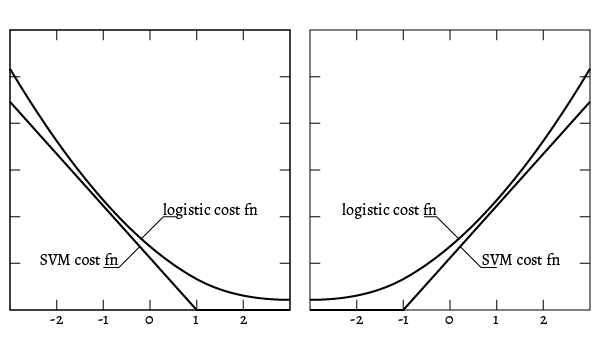
\includegraphics[height=5cm]{costfunction_logisticregressionSVM}
\caption{Cost function of logistic regression vs. SVM}
\label{fig:costfunction_logisticregressionSVM}
\end{figure}

Logistic regression:\\
   \begin{align*} 
        \min\frac{1}{m}\sum_{i=1}^m \left[ y^{(i)}(-\log(h_\theta(x^{(i)}))) + (1-y^{(i)})(-\log(1- h_\theta(x^{(i)}))) \right] + \frac{\lambda}{2m}\sum_{j=1}^n\theta_j^2
    \end{align*}
    
Support vector machine (with hinge loss function):\\
   \begin{align} 
        &\min\frac{1}{m}\sum_{i=1}^m \left[ y^{(i)}\text{cost}_1(\theta^Tx^{(i})) + (1-y^{(i)})(\text{cost}_0(\theta^Tx^{(i)}) \right] + \frac{\lambda}{2m}\sum_{j=1}^n\theta_j^2\\
        &\min C \sum_{i=1}^m \left[ y^{(i)}\text{cost}_1(\theta^Tx^{(i})) + (1-y^{(i)})(\text{cost}_0(\theta^Tx^{(i)}) \right] + \frac{1}{2}\sum_{j=1}^n\theta_j^2\\
    &\text{cost}_0 = \max(0, k(1+z)) \nonumber\\
    &\text{cost}_1 = \max(0, k(1-z)) \nonumber         
    \end{align}

Hypothesis:\\
\begin{align*}
h_\theta(x)  = \left\{ \begin{array}{rll}
         1 & \text{if} \quad \theta^Tx \geq 0\\
         0 & \text{otherwise}
                \end{array}\right.\\
\end{align*}

\emph{\textcolor{Bittersweet}{Informally, the  parameter $C$ is a positive value that controls the penalty for misclassified training examples. A large  $C$ tells the SVM to try to classify all the examples correctly.  $C$ plays a role similar to $\frac{1}{\lambda}$.}}
%
\subsection{Large margin intuition}
If $y = 1$, we want $\theta^Tx \geq 1$ (not just $\theta^Tx \geq 0$)\\
If $y = 0$, we want $\theta^Tx < -1$ (not just $\theta^Tx < 0$)\\
This builds in an extra safety factor or safety margin factor into the support vector machine.

%%
\subsubsection{SVM decision boundary}
If C is very large (e.g., 100,000), then minimizing the optimization objective leads to setting\\

$\sum_{i=1}^m \left[ y^{(i)}\text{cost}_1(\theta^Tx^{(i})) + (1-y^{(i)})\text{cost}_0(\theta^Tx^{(i)}) \right]$ to $0$:\\

Whenever $y^{(i)} = 1: \theta^Tx^{(i)} \geq 1$

Whenever $y^{(i)} = 0: \theta^Tx^{(i)} \leq -1$
\begin{align}
&\underset{\theta}{\min}\frac{1}{2}\sum_{i=1}^{n}\theta_j^2 \nonumber \\
s.t. \quad &\theta^Tx^{(i)} \geq 1, \quad \text{if} \quad y^{(i)} = 1 \nonumber \\
&\theta^Tx^{(i)} \leq -1, \quad \text{if} \quad y^{(i)} = 0
\end{align}
 
\begin{itemize}
\item
Linearly separable case (Large margin classifier)\\
a robust separator, a larger minimum distance from any of the training examples. This distance is called the \textbf{margin} of the support vector machine and this gives the SVM a certain robustness, because it tries to separate the data (positive vs. negative examples) with as large a margin as possible. 
\item
Large margin classifier in presence of outliers\\
When $C$ is not very large, SVM can do a better job ignoring the few outliers.
\end{itemize}

%% 
\subsubsection{Maths behind large marge classification}
Vector inner product:
\begin{align*}
u &= \begin{bmatrix} u_1 \\ u_2 \end{bmatrix}, v = \begin{bmatrix} v_1 \\ v_2 \end{bmatrix}\\
\|u\| &= \text{the norm or the euclidean length of the vector} ~ u.\\
&=\sqrt{u_1^2 + u_2^2} \in \mathbb{R}\\
P &= \text{the signed length of the projection of} ~ v ~ \text{on to} ~ u, P \in \mathbb{R}\\
u^{T}v &= P \cdot \|u\| = u_1v_1+u_2v_2\\
& = v^{T}u
\end{align*}
SVM decision boundary
\begin{align}
&\underset{\theta}{\min}\frac{1}{2}\sum_{i=1}^{n}\theta_j^2  \nonumber \\
&= \frac{1}{2}(\theta_1^2+\theta_2^2) = \frac{1}{2}\left(\sqrt{\theta_1^2+\theta_2^2}\right)^2 = \frac{1}{2}\|\theta\|^2\\
s.t. \quad &\theta^Tx^{(i)} \geq 1,~ \text{if} ~y^{(i)} = 1 \nonumber  \\
&\theta^Tx^{(i)} \leq -1, ~ \text{if} ~ y^{(i)} = 0 \nonumber \\
&\theta^Tx^{(i)} = p^{(i)} \cdot \|\theta\| = \theta_1x_1^{(i)} + \theta_2x_2^{(i)} \\
&\text{where} ~ p^{(i)} ~ \text{is the projection of} ~ x^{(i)} ~ \text{onto the vector} ~ \theta \nonumber \\
&\text{Simplification:} ~ \theta_0 = 0 \nonumber \\
&\text{i.e., the decision boundary must pass through the origin, (0,0)} \nonumber \\
\rightarrow & \nonumber \\
s.t. \quad &p^{(i)} \cdot \|\theta\| \geq 1, ~ \text{if} ~ y^{(i)} = 1 \nonumber \\
&p^{(i)} \cdot \|\theta\| \leq -1, ~ \text{if} ~y^{(i)} = 0 \nonumber
\end{align}
The vector for $\theta$ is perpendicular to the decision boundary. In order for the optimization objective (above) to hold true, we need the absolute value of our projections $p^{(i)}$ to be as large as possible.\\

\emph{\textcolor{Bittersweet}{The magnitude of the margin (the gap that separates positive and negative examples) is exactly the values of $p^{(i)}$. By making the projections ($p^{(i)}$) large, the SVM can end up with a smaller value for $\|\theta\|$ in the objective.}}

%
\subsection{Kernels}
%%
\subsubsection{Non-linear decision boundary}

One way to do so is to come up with a set of complex polynomial features:\\

Predict $y=1$,\\
if $\theta_0 + \theta_1x_1 + \theta_2x_2 + + \theta_3x_1x_2 + \theta_4x_1^2 + \theta_5x_2^2 + \cdots \geq 0$\\

\underline{Another notation}:\\
$\theta_0 + \theta_1f_1 + \theta_2f_2 + \theta_3f_3 + \theta_4f_4 + \cdots$, where $f_1 = x_1, f_2 = x_2, f_3 = x_1x_2, f_4 = x_1^2, \cdots$\\

Is there a different / better choice of the features $f_1, f_2, f_3, \cdots$?\\
Given $x$, compute new features depending on the proximity to landmarks $l^{(1)}, l^{(2)}, l^{(3)}$\\
\begin{align*}
\text{Given} x: \quad 
& f_1 = \text{similarity}(x, l^{(1)})=\exp{\left(-\frac{{\|x-l^{(1)}\|}^2}{2\sigma^2}\right)}\\
& f_2 = \text{similarity}(x, l^{(2)})=\exp{\left(-\frac{{\|x-l^{(2)}\|}^2}{2\sigma^2}\right)}\\
& f_3 = \text{similarity}(x, l^{(3)})=\exp{\left(-\frac{{\|x-l^{(3)}\|}^2}{2\sigma^2}\right)}\\
\end{align*}

%%
\subsubsection{Kernels and similarity}

similarity = kernel\footnote{Kernels generalize the notion of ``inner product similarity''}, i.e., $k(x, l^{(i)})$, here is Gaussian kernels. $\sigma$ determines how fast the similarity metric decreases (to 0) as the examples are further apart.\\
\begin{align}
& f_1 = \text{similarity}(x, l^{(1)})=\exp{\left(-\frac{{\|x-l^{(1)}\|}^2}{2\sigma^2}\right)} = \exp{\left(-\frac{\sum_{j=1}^n{\|x_j-l_j^{(1)}\|}^2}{2\sigma^2}\right)} \\
&\text{If} ~ x \approx l^{(1)}: \quad f_1 \approx \exp{\left(-\frac{0}{2\sigma^2}\right)} \approx 1 \nonumber \\
&\text{If} ~ x ~ \text{is far from} ~ l^{(1)}: \quad f_1 \approx \exp{\left(-\frac{\infty}{2\sigma^2}\right)} \approx 0 \nonumber
\end{align}
These features measure how similar (close) $x$ is from each of the landmarks.\\

The hypothesis given these features are:\\
Predict 1 when\\
$\theta_0 + \theta_1f_1 + \theta_2f_2 + + \theta_3f_3 \geq 0$\\
The extra features are defined using landmarks and similarity functions to learn more complex nonlinear classifier.\\

Where to get $l^{(1)}, l^{(2)}, l^{(3)}, \cdots$?\\\\
Given $(x^{(1)}, y^{(1)}), (x^{(2)}, y^{(2)}), \cdots, (x^{(m)}, y^{(m)})$,\\
choose $l^{(1)} = x^{(1)}, l^{(2)} = x^{(2)}, \cdots, l^{(m)} = x^{(m)}$.\\
Given example $x$:\\
\begin{align*}
& f_1 = \text{similarity}(x, l^{(1)})\\
& f_2 = \text{similarity}(x, l^{(2)})\\
&f = \begin{bmatrix}f_0 \\ f_1 \\ f_2 \\ \vdots \\ f_m\end{bmatrix}, f_0 = 1
\end{align*}
For training example $(x^{(i)}, y^{(i)})$:\\
\begin{align*}
f_1^{(i)} &= \text{similarity}(x^{(i)}, l^{(1)})\\
f_2^{(i)} &= \text{similarity}(x^{(i)}, l^{(2)})\\
&\vdots\\
f_i^{(i)} &= \text{similarity}(x^{(i)}, l^{(i)}) = \exp\left(-\frac{0}{2\sigma^2}\right) = 1\\
&\vdots\\
f_m^{(i)} &= \text{similarity}(x^{(i)}, l^{(m)})\\
x^{(i)} & \in \mathbb{R}^{n+1} \rightarrow f ^{(i)}= \begin{bmatrix}f_0^{(i)} \\ f_1^{(i)} \\ f_2^{(i)} \\ \vdots \\ f_m^{(i)}\end{bmatrix} \in \mathbb{R}^{m+1}\\
\end{align*}

%%
\subsubsection{SVM with kernels}

Hypothesis: Given $x$, compute features $f \in \mathbb{R}^{m+1}$

Pridict ``$y = 1$'', if $\theta^Tf \geq 0$, $\theta \in \mathbb{R}^{m+1}$

Training:
\begin{align}
\min C \sum_{i=1}^m \left[ y^{(i)}\text{cost}_1(\theta^Tf^{(i)}) + (1-y^{(i)})(\text{cost}_0(\theta^Tf^{(i)}) \right] + \frac{1}{2}\sum_{j=1}^m\theta_j^2
\end{align}

\emph{\textcolor{Bittersweet}{Note that the effective number of features is the dimension of $f$, so that the number of features $n$ is going to be equal to the number of training samples $m$. SVM uses $\theta^{T}M\theta$ instead of $\theta^T\theta$, which allows it to scale to much bigger training sets (i.e., an implementational detail, primarily for reasons of computational efficiency). The computational tricks that apply for SVM don't generalize well to other algorithms like logistic regression.}}

%%
\subsubsection{SVM bias and variance trade-offs}
\begin{itemize}
\item
$C (\approx \frac{1}{\lambda})$\\
Large C: Lower bias, high variance.\\
Small C: High bias, low variance.
\item
$\sigma^2$\\
Large $\sigma^2$: Features $f_i$ vary more smoothly. Higher bias, lower variance.\\
Small $\sigma^2$: Features $f_i$ vary less smoothly. Lower bias, higher variance.
\end{itemize}

%
\subsection{Using an SVM}
Use SVM software package (e.g., liblinear, libsvm, $\cdots$) to solve for parameters $\theta$.

Need to specify:
\begin{itemize}
\item
Choice of parameter C
\item
Chocie of kernel (similarity function)\\
\begin{itemize}
\item
No kernel (``linear kernel''):\\
Predict ``$y = 1$'', if $\theta^Tx \geq 0$. In case $n$ is large and $m$ is small, $x \in \mathbb{R}^{n+1}$
\item
Gaussian kernel:\\
$f_i = \exp{\left(-\frac{{\|x-l^{(i)}\|}^2}{2\sigma^2}\right)}$, where $l^{(i)} = x^{(i)}$. In case $n$ is small and $m$ is large, $x \in \mathbb{R}^{n+1}$\\
Need to choose $\sigma^2$.\\
Note: Do perform feature scaling before using the Gaussian kernel.\\
\item
Other choices of kernels:\\
Note: Not all similarity functions $\text{similarity}(x,l)$ make valid kernels. Need to satisfy technical condition called ``Mercer's Theorem'' to make sure SVM packages' optimizations run correctly, and do not diverge.\\
Many off-the-shelf kernels available:\\
Polynomial kernel: $k(x,l) = (x^Tl)^2, (x^Tl)^3, (x^Tl + 1)^2, (x^Tl + 5)^4, (x^Tl + \text{constant})^{\text{degree}}$, etc.\\
More esoteric: String kernel, chi-square kernel, hitogram intersection kernel, etc.
\end{itemize}
\item
Multi-class classification\\
One-vs.-all method: $y \in \{1, 2, \cdots, K\}$. Train $K$ SVMs, one to distinguish $y = i$ from the rest, for $i = 1, 2, \cdots, K$, get $\theta^{(1)}, \theta^{(2)}, \cdots, \theta^{(K)}$. Pick class $i$ with largest $(\theta^{(i)})^Tx$.
\end{itemize}

%
\subsection{Logistic regression vs. SVMs}
$n = $ number of features ($x \in \mathbb{R}^{n+1}$), $m = $ number of training examples\\
If $n$ is large (relative to $m$), e.g., $n \gg m$:

Use logistic regression, or SVM without a kernel (``linear kernel'').\\
If $n$ is small, $m$ is intermediate:

Use SVM with Gaussian kernel.\\
If $n$ is small, $m$ is large:

Create/add more features, then use logistic regression or SVM with a kernel.

%_________________________________________________________________
\section{Unsupervised learning}
\label{sec:Unsupervised learning}

\begin{itemize}
\item
Supervised learning:\\
Given a labeled training set $\{(x^{(1)}, y^{(1)}), (x^{(2)}, y^{(2)}), \cdots, (x^{(m)}, y^{(m)})\}$, to find the decision boundary that separates the positive labeled examples and the negative labeled examples.\\
$\rightarrow$ Given a set of labels to fit a hypothesis.
\item
Unsupervised learning:\\
Given data that does not have any labels. Training set: $\{x^{(1)}, x^{(2)},\cdots, x^{(m)}\}$.\\
The algorithm is to find some structure (pattern) in the data.
\end{itemize}
%
\subsection{Clustering}
Example applications: Market segmentation; Social network analysis; Organizing computer clusters; Astronomical data analysis, etc.\\

Input:
\begin{itemize}
\item
$K$ (number of clusters)
\item
Training set: $\{x^{(1)}, x^{(2)},\cdots, x^{(m)}\}$\\
$x^{(i)} \in \mathbb{R}^n$ (drop $x_0 = 1$ convention)
\end{itemize}

%%
\subsubsection{K-means algorithm}

Randomly initialize $K$ cluster centroids $\mu_1, \mu_2, \cdots, \mu_K \in \mathbb{R}^n, k \in \{1, 2, \cdots, K\}$

Repeat $\{$ \\

\emph{--Cluster assignment--}\\
\indent for $i = 1$ to $m$\\
\indent \indent $c^{(i)} :=$ index (from $1$ to $K$) of cluster centroid closest to $x^{(i)}$.\\
\indent \indent $c^{(i)} = \underset{k}{\mathrm{argmin}} \ \|x^{(i)} - \mu_k\|^2$ \\

\indent --$\text{minimize} ~ J, \text{w.r.t.}, c^{1}, c^{2}, \cdots, c^{m}, \text{holding} ~ \mu_1, \mu_2, \cdots, \mu_k$ fixed--\\

\emph{--Move centroid--}\\
\indent for $k = 1$ to $K$\\
\indent \indent $\mu_k :=$ average (mean) of points assigned to cluster $k$ \\
\indent \indent $\mu_k = \frac{1}{n}[x^{(k_1)} + x^{(k_2)} + \cdots + x^{(k_n)}] \in \mathbb{R}^n$ \\

\indent --$\text{minimize} ~ J, \text{w.r.t.}, \mu_1, \mu_2, \cdots, \mu_k$--\\
$\}$\\

K-means is also applied to data sets where there may not be several well separated clusters. K-means can still evenly segment such data into $K$ subsets, so can still be useful in this case.

\begin{itemize}
\item
    Optimization objective (distortion function):\\
    $\mu_{c^{(i)}} = $ cluster centroid of cluster to which example $x^{(i)}$ has been assigned.
    \begin{align}
    &J(c^{1}, c^{2}, \cdots, c^{m}, \mu_1, \mu_2, \cdots, \mu_k) = \frac{1}{m}\sum_{i=1}^m\|x^{(i)} - \mu_{c^{(i)}}\|^2\\
    &\min_{\substack{c^{1}, c^{2}, \cdots, c^{m} \\ \mu_1, \mu_2, \cdots, \mu_k}}{J(c^{1}, c^{2}, \cdots, c^{m}, \mu_1, \mu_2, \cdots, \mu_k)} \nonumber
    \end{align}
    With k-means, it is not possible for the cost function to sometimes increase. $J$ should always decrease as $K$ is increased.
\item
    Random initialization:
        \begin{itemize}
        \item
        Should have $K<m$
        \item
        Randomly pick $K$ training examples.
        \item
        Set $\mu_1, \mu_2, \cdots, \mu_k$ equal to these $K$ examples.
    \end{itemize}
    Try multiple random initialization to ameliorate K-means getting stuck in local optima. When the initial centroids are selected, be sure that they are each unique.\\
    for $i = 1, 2, \cdots 100$\{
    \begin{itemize}
        \item[]
        Randomly initialize K-means.
        \item[]
        Run K-means. Get $c^{1}, c^{2}, \cdots, c^{m}, \mu_1, \mu_2, \cdots, \mu_k$.
        \item[]
        Compute cost function (distortion):\\
        $J(c^{1}, c^{2}, \cdots, c^{m}, \mu_1, \mu_2, \cdots, \mu_k)$
    \end{itemize}
    \}\\
    Pick clustering that gave lowest cost $J(c^{1}, c^{2}, \cdots, c^{m}, \mu_1, \mu_2, \cdots, \mu_k)$
\item
    Choosing the number of clusters (the right value of $K$):
    The value of $K$ can be ambiguous, and hard to be decided.
    \begin{itemize}
    \item[]
    Manually by looking at visualizations, output of the clustering algorithm, etc.
    \item[]
    Elbow method (worth the shot but no necessary high expectation of it working).
    \item[]
    Evaluate K-means based on a metric for how well it performs for that later purpose.
    \end{itemize}  
\end{itemize}

%
\subsection{Dimensionality reduction}
Data compression:\\
\underline{Example}: Reduce data from 3D to 2D. $x \in \mathbb{R}^3 \rightarrow z \in \mathbb{R}^2$\\
Data visualization:\\
\underline{Example}: $x \in \mathbb{R}^{50} \rightarrow z \in \mathbb{R}^{2 ~ \text{or} ~ 3}$

%%
\subsubsection{Principal component analysis}
\underline{Example}: 
\begin{itemize}
\item
2D $\rightarrow$ 1D, find a direction (a vector $u^{(1)} \in \mathbb{R}^n$) onto which to project the data so as to minimize the projection error (i.e., the average of all the distances of every feature to the projection line).
\item
n-D $\rightarrow$ k-D, k vector ($u^{(1)}, u^{(2)}, \cdots, u^{(k)}$) onto which to project the data so as to minimize the projection error.
\end{itemize}

\emph{\textcolor{Bittersweet}{PCA is not linear regression, e.g., the ``projection error'' (i.e., shortest orthogonal distances) is different from the ``mean squared error'' (i.e., vertical distances to the label), all the features are treated symmetrically. PCA trys to find a lower dimensional surface onto which to project the data, so as to minimize the squared project error.}}

%%
\subsubsection{PCA algorithm}
Training set: $\{x^{(1)}, x^{(2)},\cdots, x^{(m)}\}$.\\
Preprocessing (feature scaling/mean normalization):
\begin{itemize}
\item
$\mu_j = \frac{1}{m}\sum_{i = 1}^mx_j^{(i)}$ (mean of each features)\\
Replace each $x_j^{i}$ with $x_j^{i} -\mu_j$ (so that each feature has zero mean)
\item
If different features on different scales, scale features to have comparable range of values.\\
$x_j^{i} \leftarrow \frac{x_j^{i} - \mu_j}{s_j}$
\end{itemize}
Reduce data from $n-$dimensions to $k-$dimensions: $x^{(i)} \in \mathbb{R}^{n \times 1} \rightarrow z^{(i)} \in \mathbb{R}^{k \times 1}$\\
Compute ``covariance matrix'':\\
\begin{align}
\Sigma = \frac{1}{m}\sum_{i=1}^n(x^{(i)})(x^{(i)})^T \in \mathbb{R}^{n \times n}
\end{align}
Compute ``eigenvectors or singular vectors '' of matrix $\Sigma$, e.g., singular value decomposition \footnote{a factorization of a real or complex matrix that generalize the eigendecomposition.} $\Sigma = USV^T, \text{here} ~ \Sigma \in \mathbb{R}^{n \times n}, \text{so} ~ U \in \mathbb{R}^{n \times n} \footnote{$U$ is a Unitary matrix, $U^{-1} = U^H$, with real numbers here so $U^{-1} = U^T$}, S \in \mathbb{R}^{n \times n} ~ \text{diagonal}, V \in \mathbb{R}^{n \times n}$.
We take the first $k$ vectors of the matrix $U \in \mathbb{R}^{n \times n}$ as $U_{\text{reduced}} \in \mathbb{R}^{n \times k}$
\begin{align}
&z^{(i)} = U_{\text{reduced}}^Tx^{(i)}\\
&X \in \mathbb{R}^{m \times n}, \Sigma = \frac{1}{m}X^TX \nonumber \\
&Z = XU_{\text{reduced}}
\end{align}

%%
\subsubsection{Reconstruction from compressed representation}
\underline{Example}: $z^{(i)}  \in \mathbb{R} \rightarrow x^{(i)}  \in \mathbb{R}^2$, go back to the original number of features and get approximations of the original data.
\begin{align}
&x_{\text{approx}}^{(i)} = U_{\text{reduced}} \cdot z^{(i)}\\
&Z \in \mathbb{R}^{m \times k} \nonumber \\
&X_{\text{approx}} = ZU_{\text{reduced}}^T
\end{align}

%%
\subsubsection{Choosing the number of PCs}
Choosing $k$ (number of principal components)
\begin{itemize}
\item[]
Average squared projection error: $\frac{1}{m}\sum_{i=1}^m\|x^{(i)} - x^{(i)}_{\text{approx}}\|^2$\\
(The difference between the original data and the projection on the lower dimensional surface).
\item[]
Total variation in the data: $\frac{1}{m}\sum_{i=1}^m\|x^{(i)}\|^2$\\
(The average distance of the training examples from the origin).
\item[]
Typically, choose $k$ to be smalles value such that\\

$\frac{\frac{1}{m}\sum_{i=1}^m\|x^{(i)} - x^{(i)}_{\text{approx}}\|^2}{\frac{1}{m}\sum_{i=1}^m\|x^{(i)}\|^2} \leq 0.01 \quad (1\%)$

(99\% of variance is retained)\\

\item[]
    Algorithm:
    \begin{itemize}
    \item[]
    Try PCA with $k = 1, 2, \cdots$
    \item[]
    Compute $U_{\text{reduced}}, z^{(1)}, z^{(2)}, \cdots, z^{(m)}, x^{(1)}_\text{approx}, x^{(2)}_\text{approx}, \cdots, x^{(m)}_\text{approx}$
    \item[]
    Check if $\frac{\frac{1}{m}\sum_{i=1}^m\|x^{(i)} - x^{(i)}_{\text{approx}}\|^2}{\frac{1}{m}\sum_{i=1}^m\|x^{(i)}\|^2} \leq 0.01$  
    \end{itemize}
    
\item[]
    Algorithm:\\
    $S$: a diagonal matrix, with the non-negative sigular values of $\Sigma$ on the diagonal, by convention $s_1 \geq s_2 \cdots \geq s_k \geq 0$\\
    \begin{itemize}
    \item[]
    $\frac{\frac{1}{m}\sum_{i=1}^m\|x^{(i)} - x^{(i)}_{\text{approx}}\|^2}{\frac{1}{m}\sum_{i=1}^m\|x^{(i)}\|^2}
    = 1 - \frac{\sum_{i=1}^k{S_{ii}}}{\sum_{i=1}^m{S_{ii}}}$  
    \item[]
    Pick smallest value of $k$ for which
    
    $\frac{\sum_{i=1}^k{S_{ii}}}{\sum_{i=1}^m{S_{ii}}} \geq 0.99$ 
    \end{itemize}
\end{itemize}

%%
\subsubsection{Supervised learning speedup}
$\{(x^{(1)}, y^{(1)}), (x^{(2)}, y^{(2)}), \cdots, (x^{(m)}, y^{(m)})\}$\\
Extract inputs:

Unlabeled dataset: $x^{(1)}, x^{(2)}, \cdots, x^{(m)} \in \mathbb{R}^{10,000}$

\indent apply PCA $\rightarrow z^{(1)}, z^{(2)}, \cdots, z^{(m)} \in \mathbb{R}^{1000}$\\
New training set:
$\{(z^{(1)}, y^{(1)}), (z^{(2)}, y^{(2)}), \cdots, (z^{(m)}, y^{(m)})\}$\\

\emph{\textcolor{Bittersweet}{PCA defines a mapping from $x$ to $z$ and this mapping should be defined by running PCA (including the feature scaling and mean normalization) only on the training set, not to the cross validation or test sets. Having found all the parameters on the training set, the same mapping can then be applied to other examples in the cv or test sets. Bad use of PCA: trying to prevent overfitting, while PCA does not consider the labels $y$. Try the full machine learning algorithm without PCA first.}}


%_________________________________________________________________
\section{Anomaly detection}
\label{sec:Anomaly detection}
Density estimation:\\
Given dataset: $\{x^{(1)}, x^{(2)}, \cdots, x^{(m)}\}$\\
Is the new example $x_\text{test}$ anomalous?\\
Define a model $p(x)$ (the probability density that the example is not anomalous)\\
$p(x_\text{test}) < \epsilon \rightarrow$ flag anomaly\\
$p(x_\text{test}) \geq \epsilon \rightarrow$ OK

%
\subsection{Anomaly detection example}
\begin{itemize}
\item
Fraud detection:
    \begin{itemize}
    \item
    $x^{(i)} =$ features of user $i$'s activities
    \item
    Model $p(x)$ from data
    \item
    Identify unusual users by checking which have $p(x) < \epsilon$ (anomaly detector flags too many anomalous examples $\rightarrow$ decrease $\epsilon$)
    \end{itemize}
\item
Manufacturing
\item
Monitoring computers in a data center.
    \begin{itemize}
    \item
    $x^{(i)} = $ features of machine $i$
    \item
    $x_1 = $ memory use, $x_2 = $ number of disk accesses/sec, $x_3 = $ CPU load, $x_4 = $ network traffic.
    \end{itemize}
\end{itemize}

%
\subsection{Gaussian distribution}
$x \in \mathbb{R}$ is a distributed Gaussian with mean $\mu$, variance $\sigma^2$.
\begin{align}
X & \sim \mathcal{N}(\mu,\,\sigma^{2})\\
p(x;\mu,\,\sigma^{2}) &= \frac{1}{\sqrt{2\pi}\sigma}\exp{(-\frac{(x-\mu)^2}{2\sigma^{2}})}
\end{align}

%%
\subsubsection{Parameter estimation}
Given the dataset: $\{x^{(1)}, x^{(2)}, \cdots, x^{(m)}\}$\\
to estimate what are the values of $\mu,\,\sigma^{2}$:
\begin{align}
\mu &= \frac{1}{m}\sum_{i=1}^mx^{(i)}\\
\sigma^{2} &= \frac{1}{m}\sum_{i=1}^m(x^{(i)}-\mu)^2
\end{align}

Maximum likelihood estimation.

%
\subsection{Anomaly detection algorithm}
Given the unlabelled training set: $\{x^{(1)}, x^{(2)}, \cdots, x^{(m)}\}, \quad x^{(i)} \in \mathbb{R}^n$
\begin{align*}
p(x) &= p(x_1\mid \mu_1,\,\sigma^{2}_1)p(x_2\mid \mu_2,\,\sigma^{2}_2)p(x_3\mid \mu_3,\,\sigma^{2}_3) \cdots p(x_n\mid \mu_n,\,\sigma^{2}_n) \\
&= \prod_{j=1}^np(x_j\mid \mu_j,\,\sigma^{2}_j)
\end{align*}
Independence assumption.

\begin{enumerate}
\item
Choose features $x_j$ that you think might be indicative of anomalous examples.
\item
Fit parameters $\mu_1, \mu_2, \cdots, \mu_n, \sigma^{2}_1, \sigma^{2}_2, \cdots, \sigma^{2}_n,$
\begin{align*}
\mu_j &= \frac{1}{m}\sum_{i=1}^mx^{(i)}_j\\
\sigma^{2}_j &= \frac{1}{m}\sum_{i=1}^m(x^{(i)}_j-\mu_j)^2
\end{align*}
\item
Given new example $x$, compute $p(x)$:
\begin{align*}
p(x)= \prod_{j=1}^np(x_j\mid \mu_j,\,\sigma^{2}_j) 
= \prod_{j=1}^n\frac{1}{\sqrt{2\pi}\sigma_j}\exp{(-\frac{(x_j-\mu_j)^2}{2\sigma_j^{2}})}:
\end{align*}
Anomaly if $p(x) < \epsilon$
\end{enumerate}

%%
\subsubsection{Developing and evaluating an anomaly detection system}
\textbf{The importance of real-number evaluation}: When developing a learning algorithm (choosing features, etc.), making decisions is much easier if we have a way of evaluating our learning algorithm.

Assume we have some labeled data, of anomalous (e.g., 20) and non-anomalous (e.g. 10000) examples. ($y = 0$ if normal, $y = 1$ if anomalous).
\begin{itemize}
\item[]
Training set (e.g., 6000 good): $x^{(1)}, x^{(2)}, \cdots, x^{(m)}$ (assume normal examples / not anomalous)\\
$\rightarrow p(x)= \prod_{j=1}^np(x_j\mid \mu_j,\,\sigma^{2}_j) $ 
\item[]
Cross validation set (e.g., 2000 good and 10 anomalous):  $\{(x^{(1)}_{\text{cv}}, y^{(1)}_{\text{cv}}), (x^{(2)}_{\text{cv}}, y^{(2)}_{\text{cv}}), \cdots, (x^{(m)}_{\text{cv}}, y^{(m)}_{\text{cv}})\}$
\item[]
Test set (e.g., 2000 good and 10 anomalous):  $\{(x^{(1)}_{\text{test}}, y^{(1)}_{\text{test}}), (x^{(2)}_{\text{test}}, y^{(2)}_{\text{test}}), \cdots, (x^{(m)}_{\text{test}}, y^{(m)}_{\text{test}})\}$
\end{itemize}

\textbf{Algorithm evaliuation}
\begin{itemize}
\item[]
    Fit model $p(x)$ on training set $x^{(1)}, x^{(2)}, \cdots, x^{(m)}$, assuming the vast majority are normal examples
\item[]
    On a cross validation/test example $x$, predict
    \begin{align*}
    y = \left\{ \begin{array}{rll}
             1 & \text{if} \quad p(x) < \epsilon \quad \text{anomaly}\\
             0 & \text{if} \quad p(x) \geq \epsilon \quad \text{normal}
                    \end{array}\right.
    \end{align*}
\item[]
    Possible evaluation metrics, see Section \ref{sec:Machine learning system design}:\\
    (Because the data is very skewed ($y = 0$ is much more common), classification accuracy would not be a good evaluation metrics)
    \begin{itemize}
    \item
    True positive, false positive, false negative, true negative
    \item
    Precision/Recall
    \item
    $F_1-$score
    \end{itemize}
\item[]
    Can also use cross validation set to choose parameter $\epsilon$.
\end{itemize}

%%
\subsubsection{Anomaly detection vs. supervised learning}

\begin{center}
\begin{tabular}{| m{7cm} | m{7cm} | }
\hline
Anomaly detection & Supervised learning\\
\hline
Very small number of positive examples ($y = 1$), typically $0-20$. Large number of negative ($y = 0$) examples & Large number of positive and negative examples.\\
\hline
Many different ``types'' of anomalies. hard for any algorithm to learn from positive examples what the anomalies look like;
future anomalies may look nothing like any of the anomalous examples we've seen so far. & Enough positive examples for algorithm to get a sense of what positive examples are like, future positive examples likely to be similar to ones in training set.\\
\hline
\end{tabular}
\end{center}

In anomaly detection, often the number of positive examples is so small that it is not possible for a learning algorithm to learn that much from them. Instead, we take a large set of negative examples and have the learning algorithm learn a lot from them. The small number of positive examples are reserved for evaluating the algorithms.

\textbf{Application}
\begin{center}
\begin{tabular}{| m{7cm} | m{7cm} | }
\hline
Anomaly detection & Supervised learning\\
\hline
Fraud detection & Email spam classification\\
\hline
Manufacturing (e.g., aircraft engines) & Weather prediction (sunny/rainy/ect.)\\
Monitoring machines in a data center & Cancer classification\\
$\vdots$ & $\vdots$ \\
\hline
\end{tabular}
\end{center}

\emph{\textcolor{Bittersweet}{If there are equal numbers of positive and negative examples, we would tend to shift all the applications to the supervised learning column. Anomaly detection only models the negative examples, whereas a supervised learning algorithm learns to discriminate between positive and negative examples, so the supervised learning algorithm will perform better when there are many positive and negative examples.}}

%%
\subsubsection{Choosing what features to use}
Sanity check: Plot the histogram of the data, to make sure that the data looks vaguely Gaussian before feeding it to the anomaly detection algorithm.\\
If the data looks non-Gaussian, play with different transformations of the data in order to make it look more Gaussian, e.g., $x \leftarrow \log(x)$, $x \leftarrow \log(x + c)$, $x \leftarrow x^{\frac{1}{2}}$,  $x \leftarrow x^{\frac{1}{3}}$.

%%
\subsubsection{Error analysis for anomaly detection}
Want:
\begin{itemize}
\item[]
$p(x)$ large for normal examples $x$.
\item[]
$p(x)$ small for anomalous examples $x$.
\end{itemize}
Most common problem:
\begin{itemize}
\item[]
$p(x)$ is comparable (e.g., both large) for normal and anomalous examples.
\end{itemize}

Look at the anomaly that the algorithm is failing to flag (finding something unusual), and use that to create some new features, so that with these new features it becomes easier to distinguish the anomalies from the good examples.
\\\\
\underline{Example}: Monitoring computers in a data center\\
Choose features that might take on unusually large or small values int he event of an anomaly.
\begin{itemize}
\item[]
$x_1 = $ memory use of computer
\item[]
$x_2 = $ number of disk accesses/sec
\item[]
$x_3 = $ CPU load
\item[]
$x_4 = $ network traffic
\end{itemize}

Create a new feature e.g., $x_5 = \frac{\text{CPU load}}{\text{network traffic}}$, $x_6 = \frac{(\text{CPU load})^2}{\text{network traffic}}$

%
\subsection{Multivariate Gaussian distribution}
$x \in \mathbb{R}^n$. Instead of model $p(x_1), p(x_2), \cdots,$ etc. separately, model $p(x)$ all in one go.

Parameters: $\mu \in \mathbb{R}^n, \Sigma \in \mathbb{R}^{n \times n}$ (covariance matrix).
\begin{align}
p(x; \mu, \Sigma) =  \frac{1}{(2\pi)^{\frac{n}{2}}|\Sigma|^{\frac{1}{2}}}\exp{(-\frac{1}{2}(x-\mu)^T\Sigma^{-1}(x-\mu))}
\end{align}
\emph{\textcolor{Bittersweet}{Note that this $p(x)$ is for a single training example. An efficient vectorized implementation with the whole training data matrix $X$ might involve summation over dot products.}}\\

Multivariate Gaussian (Normal) examples

$\mu = \begin{bmatrix}0\\0\end{bmatrix}, \Sigma = \begin{bmatrix}1 & 0\\0 & 1\end{bmatrix}$ vs.\\
\begin{itemize}
\item
$\Sigma = \begin{bmatrix}0.6 & 0\\0 & 0.6\end{bmatrix} \rightarrow$\\
narrower distribution (the concentric ellipsis shrunk a little bit)
\item
$\Sigma = \begin{bmatrix}2 & 0\\0 & 2\end{bmatrix} \rightarrow$\\
wider distribution (the variability became wider)
\item
$\Sigma = \begin{bmatrix}0.6 & 0\\0 & 1\end{bmatrix}, \Sigma = \begin{bmatrix}2 & 0\\0 & 1\end{bmatrix} \rightarrow$\\
the distribution falls off more slowly in one direction and falls off very rapidly in the other direction
\item
$\Sigma = \begin{bmatrix}1 & 0.5\\0.5 & 1\end{bmatrix}, \Sigma = \begin{bmatrix}1 & -0.8\\-0.8 & 1\end{bmatrix} \rightarrow$\\
change the off diagonal entries to model correlations between data.
\item
$\mu = \begin{bmatrix}0\\0.5\end{bmatrix}, \mu = \begin{bmatrix}1.5\\-0.5\end{bmatrix} \rightarrow$\\
change the peak of the distribution
\end{itemize}

%
\subsection{Anomaly detection using the multivariate Gaussian distribution}
Parameter fitting:
Given training set $\{x^{(1)}, x^{(2)}, \cdots, x^{(m)}\}$
\begin{enumerate}
\item
    Fit model $p(x)$ by setting
    \begin{align*}
    \mu &= \frac{1}{m}\sum_{i=1}^mx^{(i)}\\
    \Sigma &= \frac{1}{m}\sum_{i=1}^m(x^{(i)} - \mu)(x^{(i)} - \mu)^T
    \end{align*}
\item
    Given a new example $x$, compute\\
    \begin{align*}
    p(x; \mu, \Sigma) =  \frac{1}{(2\pi)^{\frac{n}{2}}|\Sigma|^{\frac{1}{2}}}\exp{(-\frac{1}{2}(x-\mu)^T\Sigma^{-1}(x-\mu))}
    \end{align*}
    Flag an anomaly if $p(x)<\epsilon$
\end{enumerate}

%%
\subsubsection{Relationship to the original model}
The original model $p(x)= \prod_{j=1}^np(x_j\mid \mu_j,\,\sigma^{2}_j)$\\
corresponds to a special case the of multivariate Gaussian distribution, by constructing
\begin{align*}
\Sigma = \left[
    \begin{array}{cccccc}
       \sigma_1^2                                  \\
      & \sigma_2^2 & & & \text{\huge0}\\
      &               & \cdot             		\\
      &       &        & \cdot                      \\
      & \text{\huge0} &  & & \cdot         \\
      &  &   &  &  & \sigma_n^2
    \end{array}
    \right]
\end{align*}
the covariance matrix sigma must have 0's on the off diagonal elements. The controus of $p(x; \mu, \Sigma)$ are axis-aligned\\

\begin{center}
\begin{tabular}{| m{7cm} | m{7cm} | }
\hline
Original model & Multivariate Gaussian\\
\hline
Manually create features to capture anomalies where $x_1, x_2$ take unusual combinations of values, e.g., $x_3 = \frac{x_1}{x_2}$ & Automatically captures correlations between features\\
\hline
Computationally cheaper (scales better to large $n$) & Computationally more expensive ($\Sigma^{-1}$)\\
\hline
Okay even if $m$ (training set size) is small & Must have $m > n$ or else $\Sigma$ is non-invertible\\
\hline
\end{tabular}
\end{center}
\emph{\textcolor{Bittersweet}{If the covariance matrix $\Sigma$ is singular or non-invertible, check for $m \gg n$, or redundant features (e.g., $x_1 = x_2, x_3 = x_4 + 5$).}}

%_________________________________________________________________
\section{Recommender systems}
\label{sec:Recommender systems}

\underline{Example}: Predicting movie ratings\\
User rates movies using zero (one) to five stars.\\
$n_u = $ number of users\\
$n_m = $ number of movies\\

Predict how the users would have rated other movies that they have not yet rated.

%
\subsection{Content-based recommender systems}
Suppose a set of features for each of the movies, e.g., $x_1$ romance, $x_2$ action, (on a scale of 0-1).\\
For each user $j$, learn a parameter $\theta^{(j)} \in \mathbb{R}^3$. Predict user $j$ as rating movie $i$ with $(\theta^{(j)} )^Tx^{(i)}$ stars.

%%
\subsubsection{Problem formulation}
$r(i, j) = 1$ if user $j$ has rated movie $i$ (0 otherwise)\\
$y^{(i,j)} = $ rating given by user $j$ to movie $i$ (defined only if $r(i, j) = 1$)\\\\
$\theta^{(j)} = $ parameter vector for user $j$\\
$x^{(i)} = $ feature vector for movie $i$\\
For user $j$, movie $i$, predicted rating: $(\theta^{(j)} )^Tx^{(i)}$\\\\
$m^{(j)} = $ number of movies rated by user $j$\\\\
To learn $\theta^{(j)} \in \mathbb{R}^{n+1}$ (parameter for user $j$):
\begin{align*}
&\min_{\theta^{(j)}}\frac{1}{2m^{(j)}}\sum_{i : r(i,j)=1}((\theta^{(j)})^Tx^{(i)} - y^{(i,j)})^2 + \frac{\lambda}{2m^{(j)}}\sum_{k=1}^n(\theta_k^{(j)})^2\\
&\text{to simplify, eliminate the constant} ~ m^{(j)} \rightarrow \\
&\min_{\theta^{(j)}}\frac{1}{2}\sum_{i : r(i,j)=1}((\theta^{(j)})^Tx^{(i)} - y^{(i,j)})^2 + \frac{\lambda}{2}\sum_{k=1}^n(\theta_k^{(j)})^2
\end{align*}
To learn $\theta^{(1)}, \theta^{(2)}, \cdots, \theta^{(n_u)}$:
\begin{align}
&J(\theta^{(1)}, \theta^{(2)}, \cdots, \theta^{(n_u)}) \nonumber\\
&= \min_{\theta^{(1)}, \theta^{(2)}, \cdots, \theta^{(n_u)}}\frac{1}{2}\sum_{j=1}^{n_u}\sum_{i : r(i,j)=1}((\theta^{(j)})^Tx^{(i)} - y^{(i,j)})^2 + \frac{\lambda}{2}\sum_{j=1}^{n_u}\sum_{k=1}^n(\theta_k^{(j)})^2 \label{eq:CF1}
\end{align}

%%
\subsubsection{Optimization algorithm}
Gradient descent update:
\begin{align*}
\theta_k^{(j)} &:= \theta_k^{(j)} - \alpha\sum_{i : r(i,j)=1} \left( (\theta^{(j)})^Tx^{(i)} - y^{(i,j)} \right) x_k^{(i)}, (\text{for} ~ k=0)\\
\theta_k^{(j)} &:= \theta_k^{(j)} - \alpha \left( \sum_{i : r(i,j)=1} \left( (\theta^{(j)})^Tx^{(i)} - y^{(i,j)} \right)x_k^{(i)} + \lambda\theta_k^{(j)}\right), (\text{for} ~ k \neq 0)
\end{align*}

%
\subsection{Collaborative filtering}
Given a dataset without knowledge of its features $\rightarrow$ feature learning (feature finders), e.g., given the user preference, to learn the movie features.
\begin{itemize}
\item[]
Given $x^{(1)}, x^{(2)}, \cdots, x^{(n_m)}$ (and movie ratings), can estimate $\theta^{(1)}, \theta^{(2)}, \cdots, \theta^{(n_u)}$.
\item[]
Given $\theta^{(1)}, \theta^{(2)}, \cdots, \theta^{(n_u)}$, can estimate $x^{(1)}, x^{(2)}, \cdots, x^{(n_m)}$.
\item[]
Back and forth process (simultaneously learn the features and the parameters):\\
$\theta ~\text{(initial random guess)} \rightarrow x \rightarrow \theta \rightarrow x \cdots$
\end{itemize}

%%
\subsubsection{Optimization algorithm}
Given $\theta^{(1)}, \theta^{(2)}, \cdots, \theta^{(n_u)}$, to learn $x^{(i)}$:
\begin{align*}
\min_{x^{(i)}}\frac{1}{2}\sum_{j : r(i,j)=1}((\theta^{(j)})^Tx^{(i)} - y^{(i,j)})^2 + \frac{\lambda}{2}\sum_{k=1}^n(x_k^{(i)})^2
\end{align*}
Given $\theta^{(1)}, \theta^{(2)}, \cdots, \theta^{(n_u)}$, to learn $x^{(1)}, x^{(2)}, \cdots, x^{(n_m)}$:
\begin{align}
\min_{x^{(1)}, x^{(2)}, \cdots, x^{(n_m)}}\frac{1}{2}\sum_{i=1}^{n_m}\sum_{j : r(i,j)=1}((\theta^{(j)})^Tx^{(i)} - y^{(i,j)})^2 + \frac{\lambda}{2}\sum_{i=1}^{n_m}\sum_{k=1}^n(x_k^{(i)})^2  \label{eq:CF2}
\end{align}

%%
\subsubsection{Collaborative filtering algorithm}
Combining Equations \ref{eq:CF1} and \ref{eq:CF2}, minimizing $x^{(1)}, x^{(2)}, \cdots, x^{(n_m)}$ and $\theta^{(1)}, \theta^{(2)}, \cdots, \theta^{(n_u)}$ simultaneously:
\begin{align}
&J(x^{(1)}, x^{(2)}, \cdots, x^{(n_m)}, \theta^{(1)}, \theta^{(2)}, \cdots, \theta^{(n_u)}) \nonumber\\
&= \frac{1}{2}\sum_{(i,j):r(i,j)=1}((\theta^{(j)})^Tx^{(i)} - y^{(i,j)})^2 + \frac{\lambda}{2}\sum_{j=1}^{n_u}\sum_{k=1}^n(\theta_k^{(j)})^2 + \frac{\lambda}{2}\sum_{i=1}^{n_m}\sum_{k=1}^n(x_k^{(i)})^2\\
&\min_{\substack{x^{(1)}, x^{(2)}, \cdots, x^{(n_m)}\\ \theta^{(1)}, \theta^{(2)}, \cdots, \theta^{(n_u)}}}J(x^{(1)}, x^{(2)}, \cdots, x^{(n_m)}, \theta^{(1)}, \theta^{(2)}, \cdots, \theta^{(n_u)})
\end{align}

\emph{\textcolor{Bittersweet}{Here $x \in \mathbb{R}^n$ and $\theta \in \mathbb{R}^n$, no need of the convention for the interception term ($x_0 = 1, \theta_0$).}}
\begin{enumerate}
    \item
        Initialize $x^{(1)}, x^{(2)}, \cdots, x^{(n_m)}, \theta^{(1)}, \theta^{(2)}, \cdots, \theta^{(n_u)}$ to small random values.
    \item
        Minimize $J(x^{(1)}, x^{(2)}, \cdots, x^{(n_m)}, \theta^{(1)}, \theta^{(2)}, \cdots, \theta^{(n_u)})$\\
        Using gradient descent (or an advanced optimizatin algorithm),\\
        e.g., for every $j = 1, 2, \cdots, n_{u}, i = 1, 2, \cdots, n_m$:
        \begin{align*}
        \theta_k^{(j)} &:= \theta_k^{(j)} - \alpha \left( \sum_{i : r(i,j)=1}\left((\theta^{(j)})^Tx^{(i)} - y^{(i,j)}\right)x_k^{(i)} + \lambda\theta_k^{(j)} \right)\\
        x_k^{(i)} &:= x_k^{(i)} - \alpha \left( \sum_{j : r(i,j)=1}\left((\theta^{(j)})^Tx^{(i)} - y^{(i,j)}\right)\theta_k^{(j)} + \lambda x_k^{(i)}\right)
        \end{align*}
    \item
        For a user with parameters $\theta$ and a movie with (learned) features $x$, predict a star rating of $\theta^Tx$.
\end{enumerate}

%%
\subsubsection{Vecotrization: low rank matrix factorization}
Predicted ratings:
\begin{align*}
&\text{Given} ~ X \in \mathbb{R}^{n_m \times n}, \Theta \in \mathbb{R}^{n_u \times n}\\
&Y = X\Theta^T\\
&\begin{bmatrix}
(\theta^{(1)})^Tx^{(1)} & (\theta^{(2)})^Tx^{(1)} & \cdots & (\theta^{(n_u)})^Tx^{(1)} \\
(\theta^{(1)})^Tx^{(2)} & (\theta^{(2)})^Tx^{(2)} & \cdots & (\theta^{(n_u)})^Tx^{(2)} \\
\vdots			 & \vdots			      & \vdots & \vdots				     \\
(\theta^{(1)})^Tx^{(n_m)} & (\theta^{(2)})^Tx^{(n_m)} & \cdots & (\theta^{(n_u)})^Tx^{(n_m)}
\end{bmatrix}
\end{align*}

\textbf{Mean normalization} as a sort of pre-processing step for collaborative filtering, e.g., take the average ratings of the movies for the prediction of an new user who hasn't yet rated any movie.

%%
\subsubsection{Finding related products}
for each product $i$, we learn a feature vector $x^{(i)} \in \mathbb{R}^{(n)}$.\\
How to find movies $j$ related to movie $i$?\\
Find the most similar movies by using $\|x^{(i)} - x^{(j)}\|$


%_________________________________________________________________
\section{Learning with large datasets}
\label{sec:Learning with large datasets}
To come up with computationally reasonable ways in large-scale ML. We mainly benefit from a very large dataset when our algorithm has high variance when $m$ is small.

%
\subsection{Stochastic gradient descent}
Batch gradient descent (looking at all the training examples at a time);\\
Stochastic gradient descent (using one single training example each time).
\begin{center}
\begin{tabular}{ p{7cm} | p{7cm}}
\hline
\textbf{Batch gradient descent} & \textbf{Stochastic gradient descent}\\
Use all $m$ examples in each iteration & Use 1 example in each iteration\\
\hline
\\
$J_{\text{train}}(\theta) = \frac{1}{2m}\sum_{i=1}^m(h_{\theta}(x^{(i)}) -y^{(i)})^2$
&
${\text{cost}}(\theta, x^{(i)}, y^{(i)}) = \frac{1}{2}(h_{\theta}(x^{(i)}) -y^{(i)})^2$
$J_{\text{train}}(\theta) = \frac{1}{m}\sum_{i=1}^m\text{cost}(\theta, x^{(i)}, y^{(i)})$\\
\\
\hline
\begin{enumerate}
    \item[]
    \item[]
	repeat until convergence \{
	\begin{align*}
	\theta_j: = \theta_j - \alpha \frac{1}{m} \underbrace{\sum_{i=1}^m (h_\theta(x^{(i)}) - y^{(i)}) x_j^{(i)}}_{\frac{\partial }{\partial \theta_j} J(\theta)}
	\end{align*}	
	(for every $j=0, \cdots, n$)
	\}
\end{enumerate}
&
\begin{enumerate}
    \item
    Randomly `shuffle' dataset
    \item
    {repeat until convergence} \{
    	\begin{align*}
    	\text{for} ~ i = 1,2, \cdots, m \{
        \end{align*}	
    	\begin{align*}
    	\theta_j: = \theta_j - \alpha \underbrace{(h_\theta(x^{(i)}) - y^{(i)}) x_j^{(i)}}_{\frac{\partial }{\partial \theta_j} {\text{cost}}(\theta, x^{(i)}, y^{(i)})}
    	\end{align*}	
    	(for every $j=0, \cdots, n$)
    	\}
    	\}
\end{enumerate}
\\
\hline
\end{tabular}
\end{center}

When the training set size $m$ is very large, stochastic gradient descent can be much faster. The cost function of batch gradient descent should go down with every iteration (assuming a well-tuned learning rate $\alpha$) but not necessarily with stochastic gradient descent. Stochastic gradient descent will be unlikely to converge at the global minimum and will instead wander around it randomly, but usually yields a result that is close enough.

%
\subsection{Mini-batch gradient descent}
Mini-batch gradient descent can sometimes be even faster than stochastic gradient descent. Instead of using all $m$ examples as in batch gradient descent, and instead of using only $1$ example as in stochastic gradient descent, we will use some in-between number of examples $b$.
\\
Use $b$ (mini-batch size, typically 2-100) examples in each iteration
\begin{enumerate}
\item
    Get $b$ examples $\{(x^{(i)}, y^{(i)}), (x^{(i+1)}, y^{(i+1)}), \cdots, (x^{(i+b-1)}, y^{(i+b-1)})$
\item
    $\theta_j := \theta_j + \alpha\frac{1}{b}\sum_{k=i}^{i+b-1}((h_\theta(x^{(k)}) - y^{(k)}) x_j^{(k)})$\\
    (for every $j=0, \cdots, n$)
\item
    $i: = i+b$
\end{enumerate}

With a good vectorizated implementation (parallelize the gradient computations over the $b$ examples), mini-batch gradient descent is likely to outperform stochastic gradient descent, though the extra parameter $b$ might take extra time.

%
\subsection{Stochastic gradient descent convergence}
%%
\subsubsection{Checking for convergence}
\begin{itemize}
\item[]
Batch gradient descent:\\
Plot $J_\text{train}(\theta)$ as a funciton of the number of iterations of gradient descent.
\item[]
Stochastic gradient descent:\\
During learning, compute ${\text{cost}}(\theta, x^{(i)}, y^{(i)}) = \frac{1}{2}(h_{\theta}(x^{(i)}) -y^{(i)})^2$ before updating $\theta$ using $(x^{(i)}, y^{(i)})$\\
Every 1000 iterations (say), plot ${\text{cost}}(\theta, x^{(i)}, y^{(i)})$ averaged over the last 1000 or so examples processed by algorithm (increase the number of examples averaged over to plot the performance $\rightarrow$ smoother line).
\end{itemize}

Learning rate $\alpha$ is typically held constant. Can slowly decrease $\alpha$ over time if we want $\theta$ to converge, e.g., $\alpha = \frac{\text{const1}}{\text{iterationNumber} + \text{const2}}, \alpha \rightarrow 0$

%
\subsection{Online learning}
With a continuous stream of users to a website, we can run an endless loop that gets $(x,y)$, where we collect some user actions for the features in $x$ to predict some behavior $y$.\\
\underline{Example}: Shipping service website where user comes, specifies origin and destination, you offer to ship their package for some asking price, and users sometimes choose to use your shipping service ($y = 1$), sometimes not ($y = 0$).\\

A learning algorithm to help us to optimize what is the asking price that we want o offer to our users?

Feature $x$ capture properties of user, of origin/destination and asking price. We want to learn $p(y = 1 | x; \theta)$ to optimize price, e.g., using logistic regression.\\

Repeat forever \{\\
\indent Get $(x, y)$ corresponding to user.\\
\indent Update $\theta$ using $(x, y)$\\
\indent\indent $\theta_j: = \theta_j - \alpha (h_\theta(x^{(i)}) - y^{(i)}) x_j^{(i)}$\\
\indent\indent $(j = 0, 1, \cdots, n)$ \}\\
Look at one example at a time, and then discard that example. The algorithm can adapt to changing user preferences.
\\\\
\underline{Example}: Product search (learning to search)\\
The problem of learning the predicted click-through rate (CTR), i.e., learning the probablility that the user click on the specific link that the algorithm offer them $p(y = 1 | x; \theta)$.
\\\\
\underline{Other example}: Choosing special offers to show user; customized selection of news articles; product recommendation; etc. 

%
\subsection{Map-reduce and data parallelism}
We can divide up batch gradient descent and dispatch the cost function for a subset of the data to many different machines so that we can train our algorithm in parallel.\\
\underline{Example}: 4x speedup. Take the training set, split it equally into 4 subsets and send the 4 subsets of the training data to 4 different computers, each computer computes the summation over one quarter of the training set, and then finally take each computer's results, send them to the centralized server which combines the results together.\\

\begin{enumerate}
\item
Split the training set into $z$ subsets corresponding to the number of machines
\item
On each machine, calculate $\sum_{i=p}^{q}(h_{\theta}(x^{(i)}) - y^{(i)})\cdot x_j^{(i)}$\\
data split staring at $p$ and ending at $q$.
\item
MapReduce takes all the dsipatched (mapped) jobs and reduce them by:\\
$\theta_j := \theta_j - \alpha \frac{1}{m}(\text{temp}_j^{(1)} + \text{temp}_j^{(2)} + \cdots + \text{temp}_j^{(z)})$\\
for all $j = 1, 2, \cdots, n$.
\end{enumerate}

Many learning algorithms are MapReduceable if they can be expressed as computing sums of functions over the training set. Linear regression and logistic regression are easily parallelizable. For neural networks, you can compute forward propagation and back propagation on subsets of your data on many machines. Those machines can report their derivatives back to a `master' server that will combine them.\\

\textbf{Multi-core machines}\\
Split the training set and send them to different cores. Some numerical linear algebra libraries can automatically parallelize their linear algebra operations across multiple cores within the machine.


\end{document}